\documentclass{article}
\usepackage{enumerate}
\usepackage{amsfonts, amscd, amsmath, amssymb}
\usepackage{graphicx}

\oddsidemargin -0.3cm
\evensidemargin 0cm
\textwidth 16.5cm
\textheight 21cm

\def\N{\mathbb N}
\def\Z{\mathbb Z}
\def\Q{\mathbb Q}
\def\R{\mathbb R}
\def\C{\mathbb C}


\title{Tema 2. Fonaments matem\`atics del Processament Digital del Senyal}
\author{{\small J.L. Lisani (UIB)}}
\date{}

\begin{document}
\maketitle

\tableofcontents

\section{An\`alisi de Fourier}
\subsection{S\`eries de Fourier}
Com ja s'ha comentat en el tema 1 l'an\`alisi de Fourier \'es una eina
b\`asica per al processament de senyals.
\newline
Les s\`eries de Fourier apareixen de manera natural en estudiar les funcions
peri\`odiques de quadrat integrable en un per\'\i ode. El conjunt d'aquestes 
funcions es denota $L^2_P(0, a)$, on $a$ \'es el per\'\i ode.

\[ L^2_P(0, a) = \{ f: \R \rightarrow \C, \quad f \quad \mathrm{de} 
\quad \mathrm{periode} \quad 
a \quad \mathrm{i} \quad \int_0^a |f(t)|^2 dt < + \infty \} \]

$L^2_P(0, a)$ \'es un espai de Hilbert 
dotat del producte escalar 
$ \langle f, g \rangle = \int_0^a f(t) \bar{g}(t) dt$
i de la norma $||f(t)||_2= (\int_0^a |f(t)|^2 dt)^\frac{1}{2} $.

La sinusoide $e_n(t)=e^{i 2 \pi n \frac{t}{a}}$ \'es un element de 
$L^2_P(0, a)$ i el conjunt dels polinomis trigonom\`etrics de grau
menor o igual a $N$ (denotat ${\cal T}_N$) \'es un subespai vectorial de 
$L^2_P(0, a)$.
\[
{\cal T}_N=\{ p(t)=\sum_{n=-N}^{+N} c_n e^{i 2 \pi n \frac{t}{a} }, 
\quad c_n \in \C \}
\]

Volem respondre a la q\"uesti\'o de si \'es possible representar qualsevol
element de $L^2_P(0, a)$ com una suma de sinusoides 
$e_n(t)=e^{2 \pi i n \frac{t}{a}}$,
\'es a dir, donat un $N$ enter fixat, podem trobar uns coeficients $x_n$
tals que $||f - \sum_{n=-N}^{N} x_n e_n ||_2$ \'es m\'\i nim?
Una vegada resposta aquesta pregunta ens demanarem qu\`e passa quan 
$N \rightarrow + \infty$.
 
\vskip 0.3 cm
Si consideram el problema des d'un punt de vista geom\`etric, es tracta de
trobar l'element $f_N$ del subespai $\cal{T}_N$ que es troba a dist\`ancia
m\'\i nima de $f$. Quan aquest element existeix es diu que \'es la {\it millor
aproximaci\'o} de $f$ dins ${\cal T}_N$.
El seg\"uent teorema ens confirma que aquest polinomi existeix i \'es \'unic.

\vskip 0.2cm
\noindent
\textbf{Teorema 1}. {\it 
Existeix un \'unic polinomi trigonom\`etric $f_N$ dins 
${\cal T}_N$ tal que $||f-f_N||_2=\mathrm{min}\{||f-p||_2, p\in {\cal T}_N \}$.
\newline
\noindent
Aquest polinomi \'es: 
\begin{equation}
\label{eq1}
f_N(t)=\sum_{n=-N}^N c_n e^{i 2 \pi n \frac{t}{a}}
\end{equation}
\noindent
on 
\begin{equation}
\label{eq2}
c_n=\frac{1}{a} \int_0^a f(t) e^{- i 2 \pi n \frac{t}{a}} dt
\end{equation}
La dist\`ancia entre aquest polinomi i $f$ \'es
\begin{equation}
\label{eq3}
||f-f_N||^2_2=||f||^2_2-a\sum_{n=-N}^N |c_n|^2
\end{equation}
}
\vskip 0.1 cm
\noindent
Per demostrar aquest teorema necessitam el seg\"uent resultat:
\vskip 0.1 cm
\noindent
\textbf{Proposici\'o 1}. {\it
Els polinomis $e_n(t)=e^{2 \pi i n \frac{t}{a}}, n \in \Z$ s\'on 
ortogonals, \'es a dir: $\langle e_n, e_m \rangle = 0$ si $m \neq n$
i $||e_n||_2=\sqrt{a}$.
}

\vskip 0.2 cm

\noindent
\underline{Dem. Teorema 1}.

La dist\`ancia de $f$ a un polinomi qualsevol de $p\in {\cal T}_N$ es calcula 
com
\[
||f-p||^2_2=||f||^2-2\mathrm{Re} \langle f, p \rangle + ||p||^2_2
\]

\noindent
$||p||^2_2$ es calcula f\`acilment amb l'ajut de la Proposici\'o 1 i resulta
que 
\[||p||^2_2=a \sum_{n=-N}^N |x_n|^2\]

\noindent
A m\'es a m\'es, 
\[\langle f, p \rangle = \sum_{n=-N}^N \bar{x}_n \langle f, e_n \rangle\]

\noindent
si definim $c_n=c_n(f)=\frac{1}{a} \langle f, e_n \rangle$

\noindent
llavors

\[ 
\begin{array}{lclc}
||f-p||^2_2 & = & ||f||^2_2 + \sum_{n=-N}^N ( -2a \mathrm{Re}[\bar{x}_n c_n] + 
a x_n \bar{x}_n ) & = \\
\\
 & = & ||f||^2_2 +a \sum_{n=-N}^N (-2 \frac{\bar{x}_n c_n + 
x_n \bar{c}_n}{2} + x_n \bar{x}_n) & = \\
\\
 & = & ||f||^2_2+a \sum_{n=-N}^N (|c_n - x_n|^2 - |x_n|^2)
\end{array}
\]

\noindent
d'aqu\'\i $ $ dedu\"\i m que el m\'\i nim de l'expressi\'o anterior s'assoleix
\'unicament quan $x_n=c_n$ i per a aquest valor tenim l'equaci\'o (\ref{eq3}). 

\begin{flushright}
$\square$
\end{flushright}

\vskip 0.3 cm
\noindent
La seg\"uent proposici\'o se dedueix inmediatament de (\ref{eq3}).
\newline
\noindent
\textbf{Proposici\'o 2 (Desigualtat de Bessel)}. {\it
\[ 
\forall N \in \N \qquad \sum_{n=-N}^N |c_n|^2 \leq 
\frac{1}{a} \int_0^a |f(t)|^2 dt
\]
}
 
\vskip 0.2 cm
\noindent
\textbf{Corol.lari}. Per a qualsevol $f \in L^2_P(0, a)$ tenim que
\[
\sum_{n=-\infty}^{+\infty} |c_n(f)|^2 \leq +\infty
\]
\noindent
i per tant $c_n(f) \rightarrow 0$ quan $|n| \rightarrow +\infty$.

\vskip 0.4 cm
\noindent
\textbf{Teorema 2}. {\it
Si $f \in L^2_P(0, a)$, el polinomi trigonom\`etric $f_N(t)$ definit per
l'equaci\'o (\ref{eq1}) tendeix cap a $f$ dins $L^2_P(0, a)$ quan 
$N \rightarrow +\infty$, \'es a dir:
\[
\int_0^a |f(t)-f_N(t)|^2 dt \rightarrow 0 \qquad \qquad \mathrm{quan}
\qquad \qquad N \rightarrow +\infty
\]
}
\noindent
La s\`erie $\sum_{n=-\infty}^{+\infty} c_n e^{2\pi i n \frac{t}{a}}$ s'anomena
{\bf s\`erie de Fourier} de $f$ i els $c_n$ definits per l'equaci\'o 
(\ref{eq2}) s\'on els {\bf coeficients de Fourier}.

\vskip 0.3cm
Una conseq\"u\`encia inmediata del teorema anterior i de la desigualtat
(\ref{eq3}) \'es la {\bf igualtat de Parseval}:

\begin{equation}
\label{eq4}
\sum_{n=-\infty}^{+\infty} |c_n|^2=\frac{1}{a} \int_0^a |f(t)|^2 dt
\end{equation}

\vskip 0.3 cm
\noindent
\textbf{Proposici\'o 3. Velocitat de converg\`encia de la s\`erie de Fourier}.
{\it Com m\'es regular \'es $f$ m\'es r\`apidament els coeficients $c_n(f)$
tendeixen cap a zero.}

\vskip 0.2 cm
\subsubsection{Converg\`encia puntual i fen\`omen de Gibbs}
\'Es important remarcar que la converg\`encia de la s\`erie de Fourier 
\'es respecte a la norma $L^2(0, a)$, \'es a dir, el resultat de la s\`erie
i la funci\'o s\'on iguals gaireb\'e per tots els punts (g.p.t), per\`o
no necess\`ariament tenim converg\`encia puntual.
El seg\"uent exemple il.lustra aquest comentari.

\vskip 0.3 cm
\noindent
{\bf Exemple}. Sigui f(t) una funci\'o peri\`odica de per\'\i ode $2\pi$
definida de la seg\"uent manera:
\[
f(t)=\lbrace  
\begin{array}{ccc}
1 & \mathrm{si} & 0 \leq t < \pi\\
-1 & \mathrm{si} & \pi \leq t < 2\pi
\end{array}
\]

\begin{figure}
\begin{center}
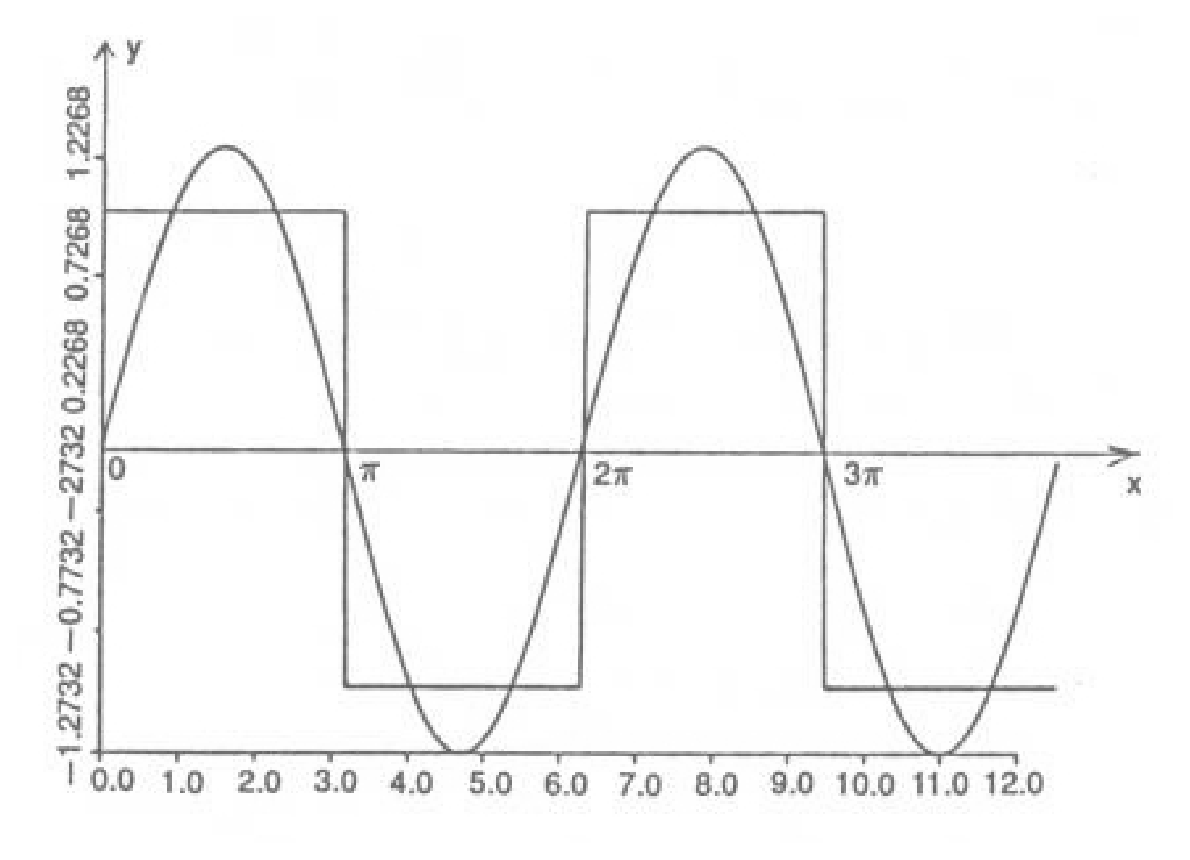
\includegraphics[width=9cm]{imatges/exserie1.eps}
\caption{[Gasquet-Witomski]. Funci\'o $f$ i $f_1(t)=\frac{4}{\pi} \sin t$}
\end{center}
\end{figure}

\begin{figure}
\begin{center}
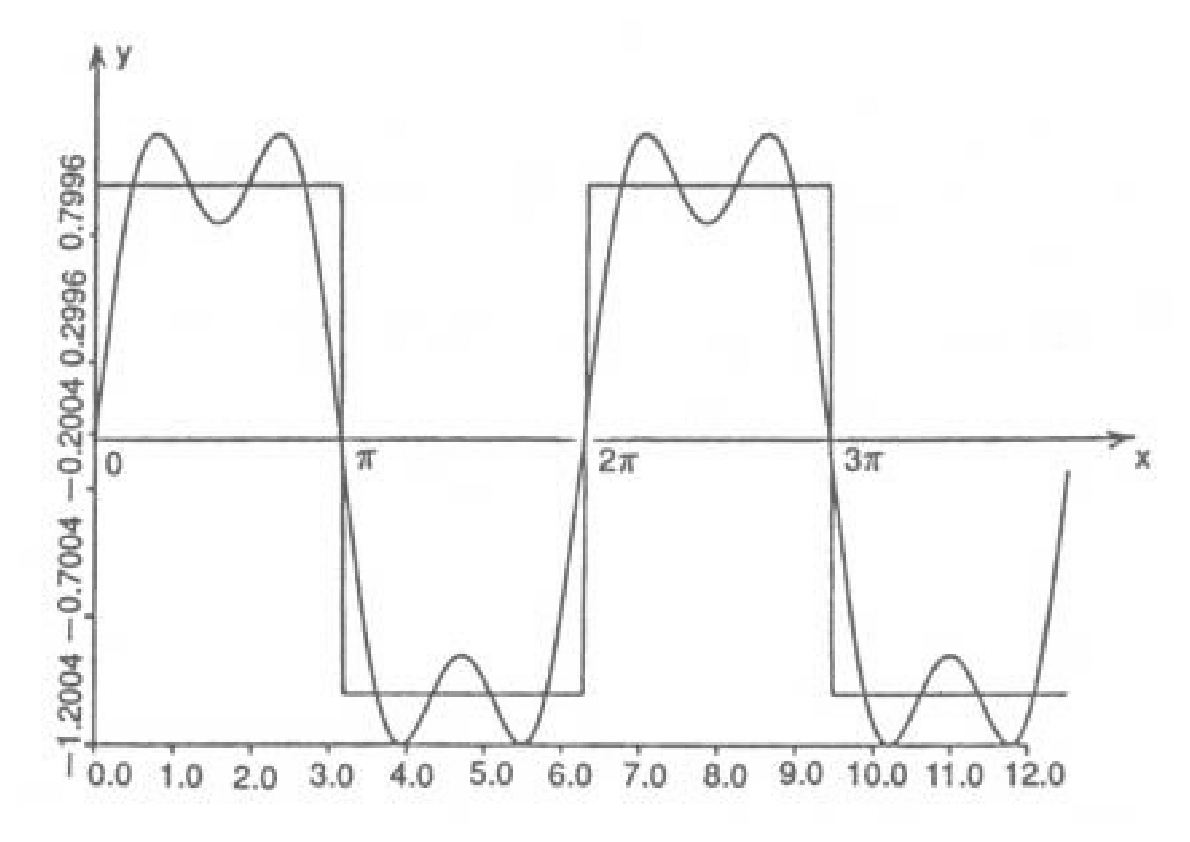
\includegraphics[width=9cm]{imatges/exserie2.eps}
\caption{[Gasquet-Witomski]. Funci\'o $f$ i 
$f_3(t)=\frac{4}{\pi} (\sin t + \frac{1}{3} \sin 3t)$}
\end{center}
\end{figure}

\begin{figure}
\begin{center}
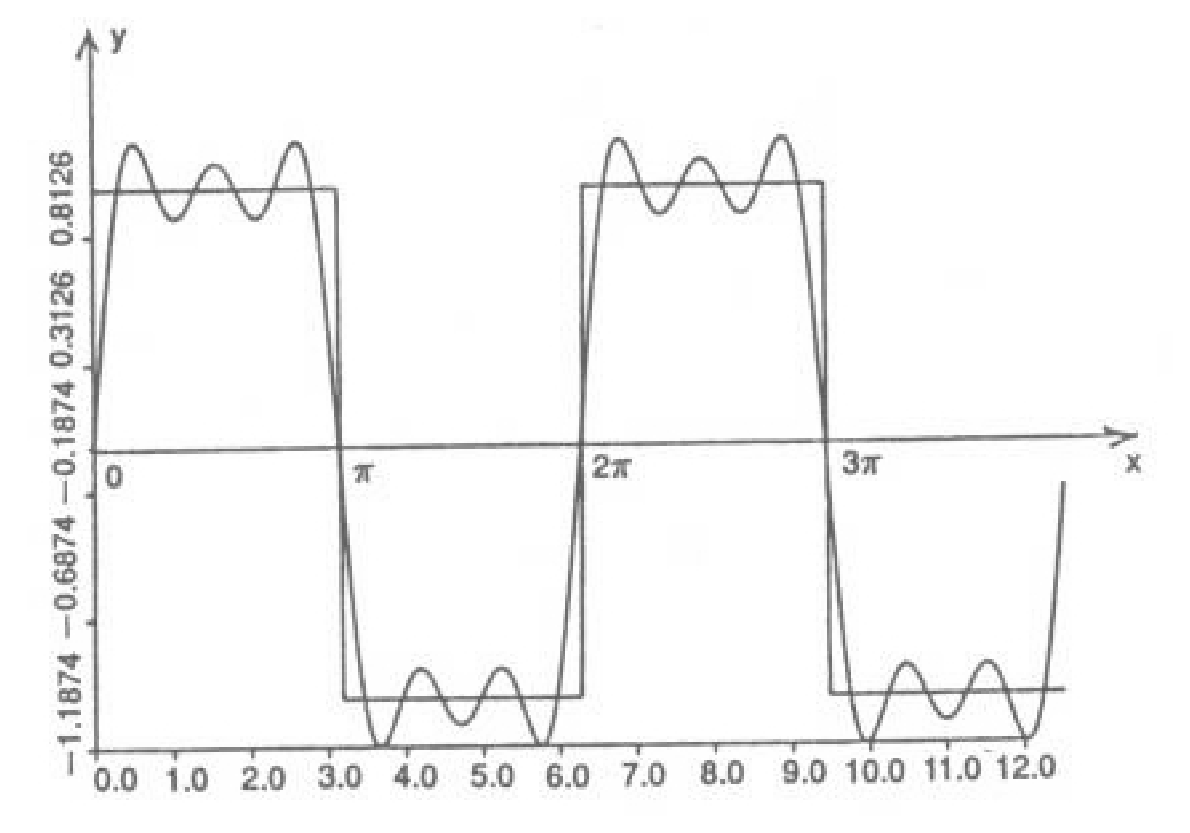
\includegraphics[width=9cm]{imatges/exserie3.eps}
\caption{[Gasquet-Witomski]. Funci\'o $f$ i
$f_5(t)=\frac{4}{\pi} (\sin t + \frac{1}{3} \sin 3t + \frac{1}{5} \sin 5t)$}
\end{center}
\end{figure}

\vskip 0.2 cm
En aquest exemple observam com $f_N(\pi)=0 \quad \forall \N$, en canvi
$f(\pi)=-1$.

\vskip 0.4 cm
El teorema seg\"uent d\'ona un resultat referent a la converg\`encia puntual
de les s\`eries de Fourier.

\noindent
\textbf{Teorema de Dirichlet o de la converg\`encia local}.{\it
Sigui $f \in L^1_P(0, a)$. Si en un punt $t_0$ els l\'\i mits 
$f(t_0+)$ i $f(t_0-)$ existeixen, aix\'\i $ $ com les derivades a dreta
i esquerra en $t_0$, llavors
\[
f_N(t) \longrightarrow \frac{1}{2} (f(t_0+)+f(t_0-)) \qquad \mathrm{quan}
\qquad N \rightarrow +\infty
\]
\noindent
(per tant $f_N(t_0) \rightarrow f(t_0)$ si $f$ \'es cont\'\i nua en $t_0$). 
}
\vskip 0.2 cm
\noindent
\textbf{Observaci\'o}. El resultat tamb\'e \'es v\`alid per a 
$f \in L^2_P(0, a)$, ja que $L^2_P(0, a) \subseteq L^1_P(0, a)$. 

\vskip 0.2 cm
\noindent
Podem comprovar que el teorema de Dirichlet es cumpleix per a la funci\'o
de l'exemple anterior.

\vskip 0.3 cm
\noindent
Un altre fen\`omen que es produeix sempre en fer un desenvolupament 
en s\`erie de Fourier d'un senyal discontinu \'es el {\bf fen\`omen de Gibbs}.
Aquest fen\`omen s'observa en les figures de l'exemple anterior: la suma de
sinusoides tendeix cap al valor de la funci\'o en els punts en qu\`e aquesta
\'es cont\'\i nua, no obstant, als voltants dels punts de discontinu\"\i itat,
la difer\`encia entre el m\`axim i el m\'\i nim de la s\`erie \'es major que
la magnitud de la discontinu\"\i tat i aquesta tend\`encia es mant\'e quan
$N \rightarrow +\infty$ (l'amplada dels ``pics'' tendeix cap a zero, per\`o
no la seva al\c{c}ada i en el l\'imit s'aproximen
a una recta vertical m\'es llarga que el bot de discontinu\"\i tat). 
\newline
Podem observar el fen\`omen de Gibbs en les figures de l'exemple anterior
i tamb\'e per a una aproximaci\'o de la funci\'o de l'exemple (amb 75 termes)
en la figura seg\"uent.

\vskip 0.1 cm

\begin{figure}[htbp]
\begin{center}
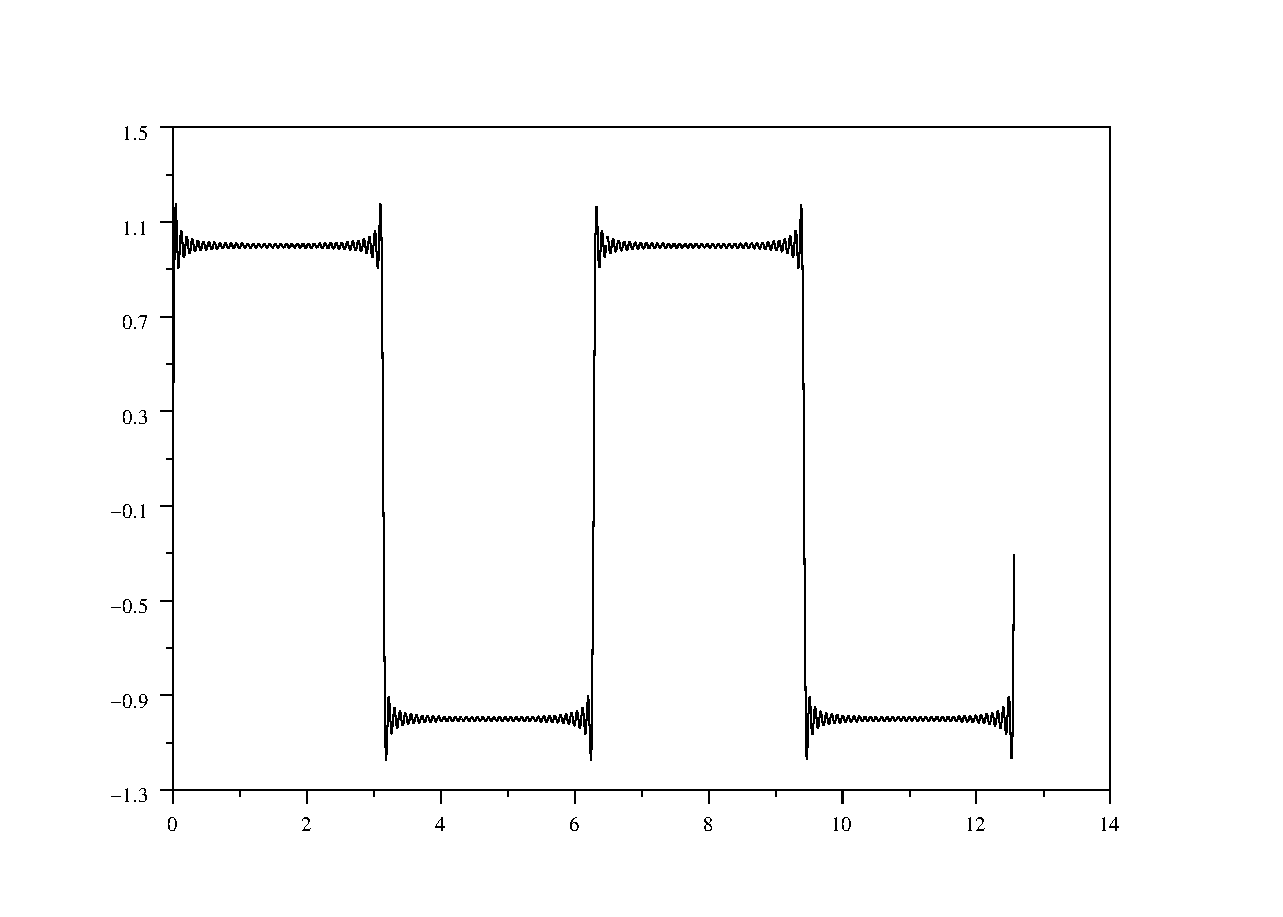
\includegraphics[width=9cm]{imatges/pulse75.eps}
\caption{Aproximaci\'o de la funci\'o de l'exemple amb 75 termes de la
s\`erie de Fourier. Observar el fen\`omen de Gibbs}.
\end{center}
\end{figure}

\subsection{An\`alisi de Fourier de funcions no peri\`odiques.
Transformades de Fourier}
L'an\`alisi de Fourier basat en desenvolupament en s\`erie t\'e un 
camp d'aplicaci\'o molt restringit i en general no es pot emprar per
estudiar els senyals obtinguts del mon f\'\i sic:
\begin{itemize}
\item els senyals tenen un suport afitat i no s'extenen des de $-\infty$ 
fins a $+\infty$
\item en general els senyals s\'on no peri\`odics
\end{itemize}
La \'unica hip\`otesi que es pot fer respecte a les propietats dels senyals
\'es que tenen una {\bf energia finita}. Si definim l'energia d'un senyal
$f(f)$ com 
\begin{equation}
\label{eqenergia}
E=\int_{-\infty}^{+\infty} |f(t)|^2 dt=||f||^2_2
\end{equation}
\noindent
la hip\`otesi implica que $E < +\infty$ i per tant $f \in L^2(\R)$.

\vskip 0.3 cm
Una manera d'obtenir una funci\'o peri\`odica i infinita a partir d'una 
funci\'o qualsevol amb suport afitat \'es mitjan\c{c}ant la 
{\bf perioditzaci\'o}.
La Figura \ref{perioditzacio.fig} mostra tres maneres possibles de fer 
aquesta perioditzaci\'o. En qualsevol dels tres casos el resultat \'es una
funci\'o que es pot desenvolupar en s\`erie de Fourier. 

\vskip 0.2 cm

\begin{figure}[htbp]
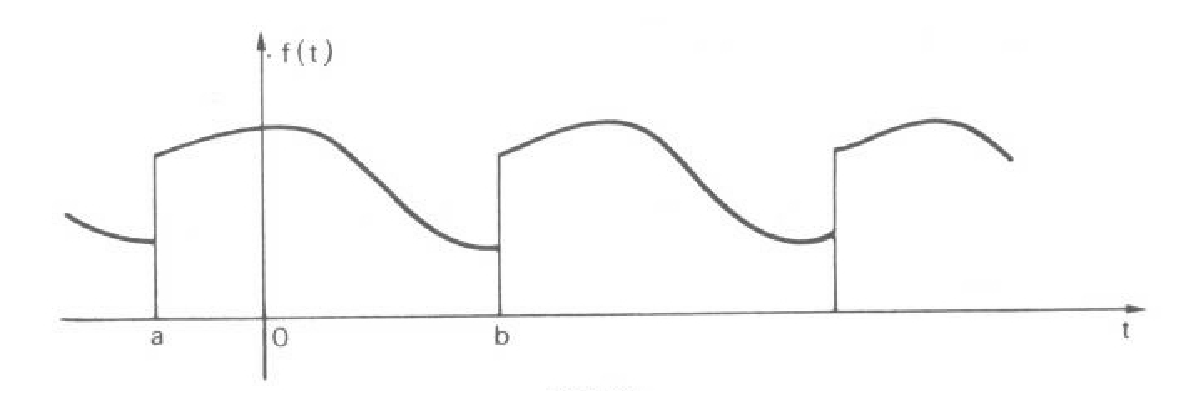
\includegraphics[width=10cm]{imatges/period1.eps}\\

\includegraphics[width=10cm]{imatges/espai.eps}\\

\includegraphics[width=10cm]{imatges/espai.eps}
\caption{Tres maneres de perioditzar una funci\'o amb suport afitat.
Dalt, perioditzaci\'o directa. Mig, simetritzaci\'o parell + perioditzaci\'o.
Baix, simetritzaci\'o imparell + perioditzaci\'o.}
\label{perioditzacio.fig}
\end{figure} 

\vskip 0.2cm
\noindent
\textbf{Observaci\'o}. La funci\'o peri\`odica obtinguda en fer una 
simetritzaci\'o imparell de la funci\'o original \'es una funci\'o imparell i 
\'es f\`acil de demostrar que la s\`erie de Fourier nom\'es cont\'e termes
en sinus. Si la perioditzaci\'o es fa despr\'es d'una simetritzaci\'o 
parell la s\`erie estar\`a composta per cosinus. Cal destacar que en aquest 
cas s'aconsegueix una funci\'o m\'es regular (sense discontinu\"\i tats de bot)
i la s\`erie de Fourier convergeix m\'es r\`apidament que en els casos 
anteriors.

\subsubsection{Transformada de Fourier}
L'extensi\'o del desenvolupament en s\`erie de Fourier a funcions 
no peri\`odiques d\'ona lloc a les Transformades (integrals) de Fourier.
La idea intuitiva del proc\'es que permet passar de les s\`eries a les 
integrals de Fourier s'esbo\c{c}a en els seg\"uents passos:
\begin{enumerate}
\item partim una funci\'o $f$ amb suport afitat entre $-\frac{a}{2}$
i $\frac{a}{2}$.
\item consideram la funci\'o peri\`odica $f_P$, de per\'\i ode $a$
que coincideix amb $f$ en l'interval $[-\frac{a}{2}, \frac{a}{2}]$.
\item desenvolupam $f_P$ en s\`erie de Fourier:
\[
f_P(t)=\sum_{n=-\infty}^{\infty} c_n e^{i2\pi\frac{n}{a}t}
\]
\[
c_n=\frac{1}{a} \int_{-\frac{a}{2}}^{\frac{a}{2}} f_P(t)
e^{-i2\pi\frac{n}{a}t} dt
\]
\item ara feim tendir $a$ cap a $+\infty$. De manera inmediata tenim que
$\lim_{a \rightarrow +\infty} f_P(t)=f(t)$.
\item si denotam $\xi_n=\frac{n}{a}$, llavors 
$\Delta \xi = \xi_{n+1}-\xi_n=\frac{n+1}{a}-\frac{n}{a}=\frac{1}{a}$.
Per tant quan $a \rightarrow +\infty$, $\Delta \xi \rightarrow d\xi$ i
el conjunt de valors discrets $\xi_n$ tendeix cap a un conjunt de valors
continus ($\xi_n \rightarrow \xi$).
\item a partir de l'expressi\'o dels coeficients de fourier podem escriure
\[
a c_n=\int_{-\frac{a}{2}}^{\frac{a}{2}} f_P(t)
e^{-i2\pi\xi_n t} dt
\]
\noindent
quan $a \rightarrow +\infty$, el segon membre d'aquesta igualtat tendeix 
cap a la integral
\[
\int_{-\infty}^{+\infty} f(t) e^{- i 2\pi \xi t} dt
\]
\noindent
si aquesta integral \'es finita (aix\'o passar\`a si 
$\int_{-\infty}^{+\infty} |f(t)| dt < +\infty$, \'es a dir,
si $f \in L^1(\R)$), tindrem que 
$\lim_{a \rightarrow +\infty} a c_n < +\infty$. Al valor d'aquest 
l\'\i mit se l'anomena {\bf transformada de Fourier} de $f$, i se
denota $\hat{f}(\xi)$.
\begin{equation}
\label{FT}
\hat{f}(\xi)=\int_{-\infty}^{+\infty} f(t) e^{-i 2\pi \xi t} dt
\end{equation}
\item el desenvolupament en s\`erie de Fourier de $f_P$ el podem reescriure
com
\[
f_P(t)=\sum_{n=-\infty}^{+\infty} (a c_n) e^{i 2 \pi \xi_n t} \frac{1}{a} =
 \sum_{n=-\infty}^{+\infty} (a c_n) e^{i 2 \pi \xi_n t} \Delta \xi
\]
\noindent
quan $a \rightarrow +\infty$ tenim que $a c_n \rightarrow \hat{f}(\xi)$,
$\xi_n \rightarrow \xi$, $\Delta \xi \rightarrow d\xi$ i 
$\sum \rightarrow \int$, per tant:
\begin{equation}
\label{IFT}
f(t)=\lim_{a \rightarrow +\infty} f_P(t)=\int_{-\infty}^{+\infty}
\hat{f}(\xi) e^{i 2 \pi \xi t} d\xi
\end{equation}
\noindent
Aquesta equaci\'o es coneix com {\bf transformada inversa de Fourier}.
(Cal assenyalar que aquesta no \'es una demostraci\'o formal de l'equaci\'o).
\end{enumerate}


\vskip 0.3 cm
\noindent
\textbf{Observacions}. 
\begin{itemize}
\item Notaci\'o. La transformada de Fourier d'una funci\'o $f$ se denota 
indistintament com $\hat{f}$ o ${\cal F} f$. La transformada inversa se
denota com ${\cal F}^{-1}$.
\item Com ja s'ha comentat m\'es amunt, la transformada de Fourier 
nom\'es pot calcular-se, en principi, per a funcions $f \in L^1(\R)$.
De la mateixa manera, la integral (\ref{IFT}) nom\'es es pot calcular
quan $\hat{f} \in L^1(\R)$.
No obstant aix\'o, \'es possible extendre les definici\'o de transformada
de Fourier i de transformada inversa de Fourier a les funcions de $L^2(\R)$
mitjan\c{c}ants arguments de densitat. 
\item Per a funcions de
$L^2(\R)$ se cumpleix que ${\cal F}^{-1}({\cal F}(f))=f$ g.p.t., en canvi aix\'o no
\'es cert en general si $f \in L^1(\R)$, ja que $\hat{f}$ pot no pert\`anyer a 
$L^1(\R)$.
\end{itemize}

\vskip 0.2 cm
A continuaci\'o se presenten alguns importants resultats relatius a les
transformades de Fourier.

\noindent
\textbf{Teorema (Riemann-Lebesgue)}.{\it 
Donada una funci\'o $f \in L^1(\R)$, es cumpleix:
\begin{itemize}
\item $\hat{f}$ \'es una funci\'o cont\'\i nua i afitada en $\R$.
\item $||\hat{f}||_{\infty}=\sup_{\xi \in \R} \hat{f}(\xi) \leq 
||f||_1=\int_{-\infty}^{+\infty} |f(t)| dt$
\item $\lim_{|\xi| \rightarrow +\infty} |\hat{f}(\xi)|=0$
\end{itemize}
}

\noindent
\textbf{Corol.lari}. Si $\hat{f} \in L^1(\R)$ llavors $f$ \'es cont\'\i nua i afitada.

\vskip 0.2 cm
\noindent
\textbf{Proposici\'o (Igualtat de Plancherel-Parseval)}.
Si $f \in L^2(\R)$ llavors:
\begin{enumerate}[i)]
\item 
\begin{equation}
\label{eq7}
\int_{-\infty}^{+\infty} f(t) \bar{h}(t) dt = \int_{-\infty}^{+\infty} \hat{f}(\xi)
\bar{\hat{h}}(\xi) d\xi
\end{equation}
\item 
\begin{equation}
\label{eq8}
\int_{-\infty}^{+\infty} |f(t)|^2 dt = \int_{-\infty}^{+\infty} |\hat{f}(\xi)|^2 d\xi
\end{equation}
\end{enumerate}

\noindent
Aquesta darrera igualtat implica que l'energia d'un senyal es pot calcular b\'e directament
a partir del senyal, b\'e a partir de la seva transformada de Fourier. A m\'es a m\'es 
ens diu que per a una funci\'o de $L^2(\R)$ $\int_{-\infty}^{+\infty} |\hat{f}(\xi)|^2 d\xi
< +\infty$.


\vskip 0.3 cm
La seg\"uent taula resumeix les propietats m\'es importants de les transformades 
de Fourier (les propietats s\'on v\`alides si $f \in L^1(\R)$ o $f \in L^2(\R)$).

\vskip 0.3 cm
\begin{tabular}{rcl}
{\bf Propietat}          & {\bf Funci\'o}        & {\bf Transformada de Fourier}\\
                         &  $f(t)$               & $\hat{f}(\xi)$\\
Inversa                  &  $\hat{f}(t)$         & $f(-\xi)$\\
Translaci\'o             &  $f(t-u)$             & $e^{-i2\pi \xi u} \hat{f}(\xi)$\\
Modulaci\'o              &  $e^{i2\pi u t} f(t)$ & $\hat{f}(\xi-u)$\\
Canvi d'escala           &  $f(t/s)$             & $|s| \hat{f}(s \xi)$\\
Derivades temporals      &  $f^{(k)}(t)$         & $(i2\pi \xi)^k \hat{f}(\xi)$\\
Derivades freq\"uencials &  $(-i2\pi t)^k f(t)$  & $\hat{f}^{(k)}(\xi)$\\
Complexe conjugat        &  $\bar{f}*(t)$      & $\bar{\hat{f}}(-\xi)$\\
Simetria hermitiana      &  $f(t) \in \R$        & $\hat{f}(-\xi)=\bar{\hat{f}}(\xi)$\\
                         &  parell               & parell\\
                         &  imparell             & imparell\\
                         &  real parell          & real parell\\
                         &  real imparell        & imagin\`aria imparell\\
\end{tabular} 

\vskip 0.5 cm
\noindent
\textbf{Teorema. Principi d'incertesa}.
Sigui $f$ una funci\'o de $L^2(\R)$.
Si definim la dispersi\'o o varian{c}a d'energia d'una funci\'o en temps 
($\sigma_t$) i en freq\"u\`encia ($\sigma_\xi$) mitjan\c{c}ant les equacions 
(\ref{eq10}) 
i (\ref{eq11}) respectivament, resulta que
\begin{equation}
\label{eq9}
\sigma_t \sigma_\xi \geq \frac{1}{4 \pi}
\end{equation}
\begin{equation}
\label{eq10}
\sigma^2_t=\frac{1}{||f(t)||^2_2}\int_{-\infty}^{+\infty} (t-t_0)^2 |f(t)|^2 dt
\end{equation}
\begin{equation}
\label{eq11}
\sigma^2_\xi=\frac{1}{||f(t)||^2_2}\int_{-\infty}^{+\infty} (\xi-\xi_0)^2 |\hat{f}(\xi)|^2 dt
\end{equation}
\noindent
$t_0$ i $\xi_0$ s\'on els valors mitjos de la funci\'o en temps i freq\"u\`encia:
\[
t_0=\frac{1}{||f(t)||^2_2}\int_{-\infty}^{+\infty} t |f(t)|^2 dt
\]
\[
\xi_0=\frac{1}{||f(t)||^2_2}\int_{-\infty}^{+\infty} \xi |\hat{f}(\xi)|^2 d\xi
\]

\vskip 0.3 cm
El que ens diu el principi d'incertesa \'es que \'es impossible tenir  
una funci\'o amb suport petit en temps i freq\"u\`encia simult\`aniament. 
Una funci\'o limitada en temps tendr\`a una amplada d'espectre (suport de la
seva transformada de Fourier) gran. I rec\'\i procament, una funci\'o amb un 
espectre petit tendr\'a una duraci\'o gran. El m\'inim de la desigualtat (\ref{eq7})
s'aconsegueix per a la funci\'o gaussiana.

\vskip 0.3 cm
A continuaci\'o es presenten tres exemples cl\`assics del c\`alcul de la Transformada
de Fourier.

\vskip 0.2 cm
\subsubsection{Exemples}
\begin{enumerate}[Exemple 1]
\item $f(t)={\cal X}_{[-a, a]}$ (funci\'o indicatriu)
\[
\hat{f}(\xi)=\int_{-a}^{a} e^{- i 2 \pi \xi t} dt = \frac{sin(2\pi a \xi)}{\pi \xi}
\]

\begin{figure}[htbp]
\begin{center}
\includegraphics[width=9cm]{imatges/sincPi.eps}
\caption{Funci\'o $\frac{sin(2 \pi a \xi)}{\pi \xi}$, amb $a=\pi$.}
\end{center} 
\end{figure}

\item $\hat{f}(\xi)={\cal X}_{[-\xi_0, \xi_0]}$ (filtre passa baix ideal)
\[
f(t)=\int_{-\xi_0}^{\xi_0} e^{i 2\pi \xi t} d\xi=
\frac{sin(2 \pi \xi_0 t)}{\pi t}
\]
\item $f(t)=e^{-a t^2}, a > 0$ (gaussiana)
\[
\hat{f}(\xi)=\sqrt{\frac{\pi}{a}} e^{-\frac{\pi^2}{a} \xi^2}
\]
\end{enumerate} 

\subsubsection{Transformada de Fourier en 2D}
\label{TFbidimensional}
Les f\`ormules per al c\`alcul de les transformades directa i inversa
de Fourier s'extenen directament a 2 dimensions.

La transformada de Fourier d'una funci\'o integrable $f(x,y) \in L^1(\R^2)$
de dues variables \'es
\begin{equation}
\label{TF2D}
\hat{f}(\xi_1,\xi_2)=\int_{-\infty}^{+\infty} \int_{-\infty}^{+\infty} 
f(x,y) e^{-i 2 \pi (\xi_1 x+\xi_2 y)} dx dy
\end{equation}

Si $\hat{f} \in L^1(\R^2)$, la transformada inversa se calcula com
\begin{equation}
\label{ITF2D}
f(x,y)=\int_{-\infty}^{+\infty} \int_{-\infty}^{+\infty} 
\hat{f}(\xi_1,\xi_2) e^{i 2 \pi (\xi_1 x+\xi_2 y)} d\xi_1 d\xi_2
\end{equation}

\vskip 0.3 cm
\noindent
{\bf Propietats}.
\begin{itemize}
\item {\bf Convoluci\'o}. Si definim 
\[
g(x, y)=(f * h)(x,y)= \int_{-\infty}^{+\infty} \int_{-\infty}^{+\infty} 
f(u, v) h(x-u,y-v) du dv
\]
\noindent
llavors $\hat{g}(\xi_1,\xi_2)=\hat{f}(\xi_1,\xi_2) \hat{h}(\xi_1,\xi_2)$.

\item {\bf Igualtat de Plancherel}.
\[
\int_{-\infty}^{+\infty} \int_{-\infty}^{+\infty} |f(x,y)|^2 dx dy=
\int_{-\infty}^{+\infty} \int_{-\infty}^{+\infty} 
|\hat{f}(\xi_1,\xi_2)|^2 d\xi_1 d\xi_2
\]

\item {\bf Rotaci\'o}. Si s'aplica a $f(x,y)$ una rotaci\'o amb un angle
$\theta$ en el pl\`a $x-y$:
\[
f_\theta(x,y)=f(x \cos\theta-y \sin\theta, x\sin\theta+y\cos\theta)
\]
\noindent
llavors la seva transformada de Fourier tamb\'e queda sotmesa a una rotaci\'o
amb el mateix angle:
\[
\hat{f}_\theta(\xi_1,\xi_2)=\hat{f}(\xi_1 \cos\theta-\xi_2 \sin\theta, 
\xi_1 \sin\theta+\xi_2 \cos\theta)
\]

\end{itemize}

\subsection{Inconvenients de les transformades de Fourier. Ondetes}
El principal inconvenient pr\`actic de l'an\`alisi de Fourier \'es que
ens proporciona una informaci\'o {\it global} del comportament dels senyals. 
Aix\'o significa que, si per exemple un senyal te una discontinuitat
brusca en un moment determinat, l'an\`alisi de Fourier ens dir\`a
que existeixen coeficients per a freq\"encies altes, per\`o no 
ens informar\`a de en quin moment s'han produ\"\i t aquestes
altes freq\"u\`encies. Nom\'es la reconstrucci\'o del senyal
original a partir dels coeficients de Fourier ens proporcionar\`a
aquesta informaci\'o.
\newline
En els darrers anys s'ha desenvolupat i popularitzat una nova eina
d'an\`alisi de les funcions que ens permet localitzar la informaci\'o
del seu comportament ent temps i freq\"u\`encia. Estam parlant de
l'an\`alisi amb {\bf ondetes} o {\bf \it wavelets}.  

\vskip 0.2 cm

\begin{figure}[htbp]
\begin{center}
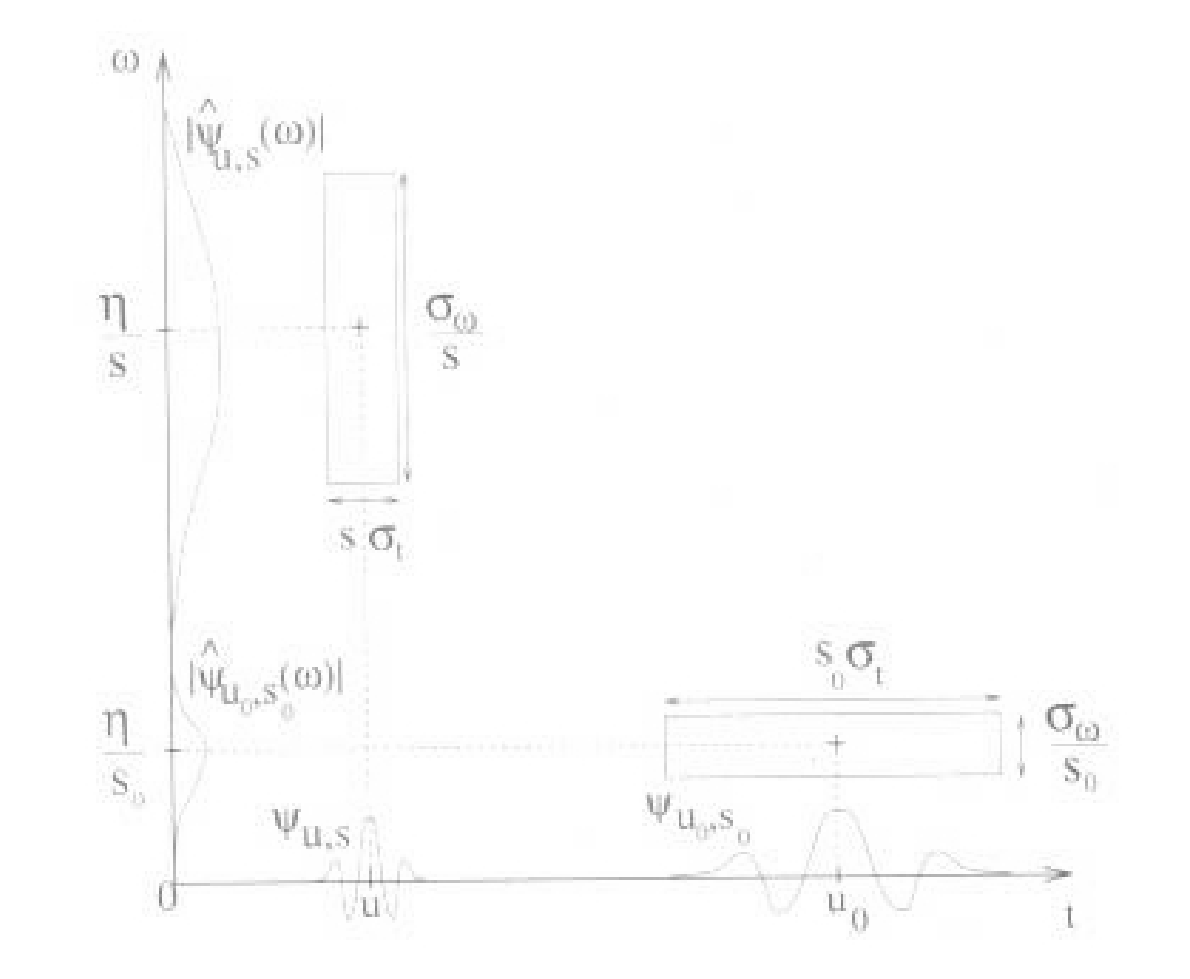
\includegraphics[width=10cm]{imatges/tempsfrequencia.eps}
\caption{[Mallat]. An\`alisi en temps i freq\"u\`encia mitjan\c{c}ant 
les ondetes.}
\end{center}
\end{figure}

\newpage
\section{Discretitzaci\'o de senyals continus}
La discretitzaci\'o d'una funci\'o cont\'\i nua implica agafar 
un conjunt finit de valors o mostres del recorregut de la funci\'o.
Aquest proc\'es s'anomena {\bf discretitzaci\'o} i el conjunt de 
valors resultant conformen una {\bf funci\'o discreta}.

Una manera de definir les funcions discretes \'es enumerant la seq\"u\`encia
de valors que pren cada una de les mostres obtingudes de la funci\'o 
cont\'\i nua original. Per exemple:

\[
f[0]=2, \quad f[1]=3, \quad f[2]=7, \quad \cdots
\]

\noindent
La notaci\'o $f[i]$ representa el valor de la $i$-\`essima mostra de la 
funci\'o.

\vskip 0.2 cm
La seg\"uent figura mostra la manera habitual de representar gr\`aficament
les funcions discretes.

\begin{figure}[htbp]
\begin{center}
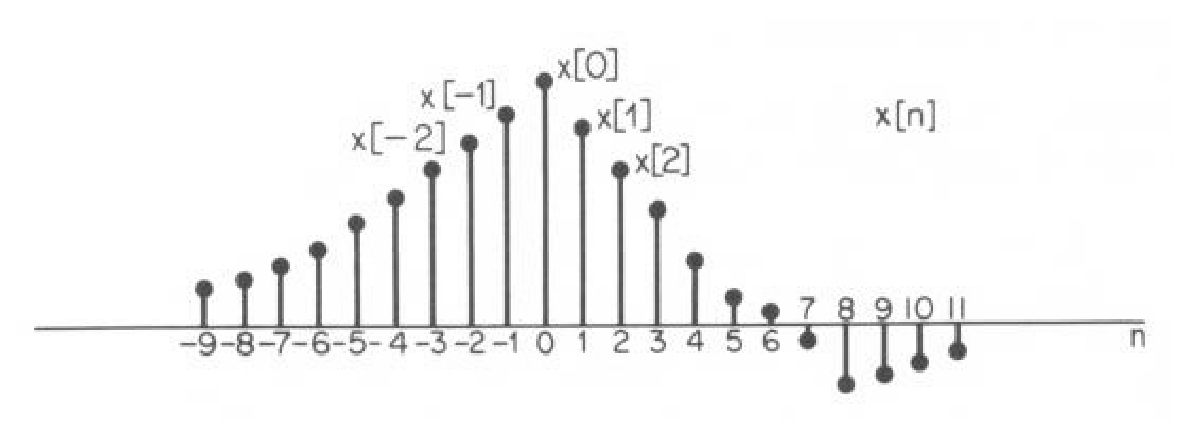
\includegraphics[width=9cm]{imatges/senyaldiscret.eps}
\caption{[Oppenheim]. Representaci\'o gr\`afica d'una funci\'o discreta}
\end{center}
\end{figure}

\vskip 0.3 cm
Habitualment la dist\`ancia (en el domini de la funci\'o) entre les mostres
consecutives es mant\'e constant durant tot el proc\'es de discretitzaci\'o
i reb el nom de {\bf per\'\i ode de mostreig}. En aquests casos les funcions 
discretes es poden definir f\`acilment a partir de les funcions originals:

\[
f[n]=f(nT) \quad \forall n \in \Z
\]

\noindent
on $T$ \'es el per\'\i ode de mostreig.
 
\vskip 0.2 cm
Una tercera manera de definir una funci\'o discreta, m\'es \'util 
per a l'estudi de les seves propietats, \'es a partir de la interacci\'o
de la funci\'o cont\'\i nua original amb unes ``funcions'' anomenades
``deltes de Dirac''. Aquesta interacci\'o es realitza, a nivell freq\"uencial,
 mitjan\c{c}ant una operaci\'o de convoluci\'o.
\newline
En la seg\"uent secci\'o es defineix l'operaci\'o de convoluci\'o entre
funcions i a continuaci\'o s'estudien les propietats de les deltes de Dirac,
les quals es definiran com un cas particular d'uns operadors de funcions 
anomenats {\bf distribucions}.


\subsection{Convoluci\'o de funcions}
\noindent
\textbf{Definici\'o}. Donades dues funcions de $\R$ en $\C$, anomenam
{\bf convoluci\'o} de $f$ i $g$ la funci\'o $f * g$, si existeix, 
definida com:
\[
f * g \, (x)=\int_{-\infty}^{+\infty} f(x-t) g(t) dt =
\int_{-\infty}^{+\infty} f(u) g(x-u) du
\]

\vskip 0.2 cm
\noindent
\textbf{Exemple}. Anam a calcular la convoluci\'o de les funcions
$f(x)=g(x)={\cal X}_{[0, 1]}$.
\[
f * g \, (x) = \int_0^1 {\cal X}_{[0, 1]} (x-t) dt = 
\begin{cases} 
0    & \mathrm{si} \quad x \leq 0\\
x    & \mathrm{si} \quad 0 < x \leq 1\\
2-x  & \mathrm{si} \quad 1 < x \leq 2\\
0    & \mathrm{si} \quad x \geq 2
\end{cases}
\]

\noindent
La Figura \ref{figpulse.fig} mostra les funcions inicials 
i el resultat de la convoluci\'o.  

\begin{figure}[htbp]
\begin{center}
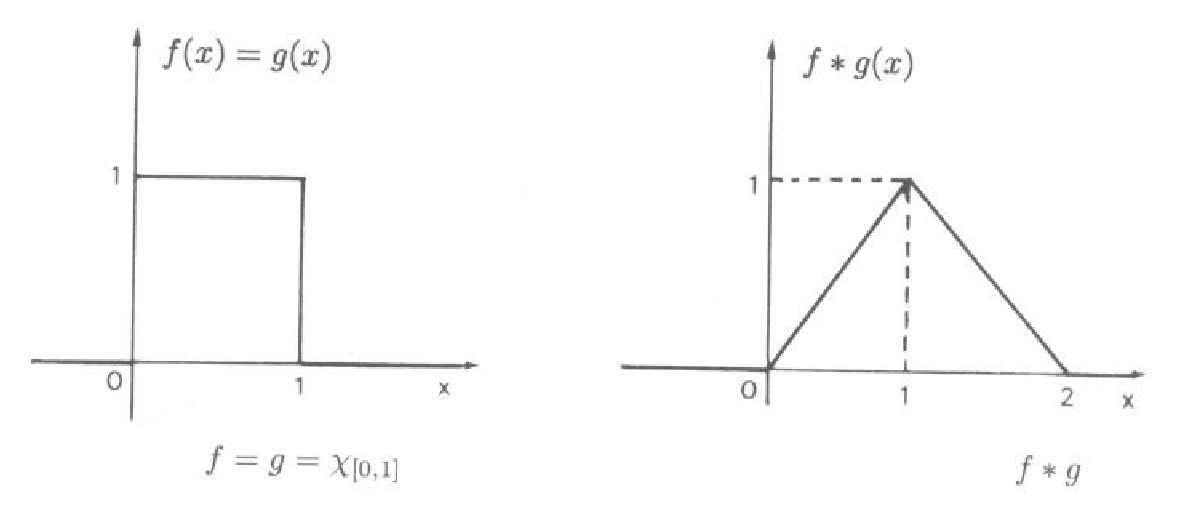
\includegraphics[width=9cm]{imatges/exconvolucio.eps}
\caption{[Gasquet-Witomski]. Funci\'o $f(x)=g(x)={\cal X}_{[0, 1]}$ i 
resultat de $f * g$.}
\end{center}
\label{figpulse.fig}
\end{figure}

\vskip 0.2 cm
En aquest senzill exemple podem apreciar dues importants propietats de la
convoluci\'o:
\begin{itemize}
\item la convoluci\'o de dues funcions discontinues \'es cont\'\i nua
\item el suport de la convoluci\'o de $f * g$ est\'a contingut en la suma 
dels suports de les funcions $f$ i $g$
\end{itemize}
\noindent
En general podem dir que la convoluci\'o \'es una operaci\'o que 
{\it regularitza} i ext\'en el domini de les funcions amb les quals opera.
    
\vskip 0.2 cm
La seg\"uent taula resum els resultats relatius a la convoluci\'o de 
diferents tipus de funcions:

\vskip 0.2 cm

\begin{center}
\begin{tabular}{lcl}
  $L^1 * L^1$                  & $\longrightarrow$ & $L^1$ \\
  $L^1 * L^\infty$             & $\longrightarrow$ & 
$L^{\infty} \cap {\cal C}^0$ \\
  $L^2 * L^2$                  & $\longrightarrow$ & 
$L^\infty \cap {\cal C}^0$ \\
  $L^2 * L^1$                  & $\longrightarrow$ & 
$L^2$ \\
  ${\cal C}^0_c *{\cal C}^0_c$ & $\longrightarrow$ & ${\cal C}^0_c$
\end{tabular}
\end{center}

\vskip 0.3 cm
\noindent
On $L^1=L^1(\R)$, $L^2=L^2(\R)$, $L^\infty=L^\infty(\R)$ i 
${\cal C}^0_c$ fa refer\`encia a les funcions continues amb suport afitat 

\vskip 0.3 cm
La seg\"uent proposici\'o \'es molt important perqu\`e relaciona la 
convoluci\'o de funcions amb la transformada de Fourier.
\newline
\noindent
\textbf{Proposici\'o}.
Donades dues funcions $f$ i $g$ de $L^1(\R)$, tenim que 
\[
{\cal F} ( f * g ) (\xi) = \widehat{f * g}(\xi)=
\hat{f} (\xi) \cdot \hat{g} (\xi)={\cal F} f (\xi) \cdot {\cal F} g (\xi)
\]
\noindent
si a m\'es $\hat{f}$ i $\hat{g}$ s\'on de $L^1(\R)$, llavors:
\[
{\cal F} ( f \cdot  g ) (\xi) = \widehat{f \cdot g}(\xi)=
\hat{f} (\xi) * \hat{g} (\xi)={\cal F} f (\xi) * {\cal F} g (\xi)
\]

\vskip 0.2 cm
\noindent
Aquestes propietats es poden extendre per a funcions de $L^2(\R)$, emprant
arguments relatius a la densitat de les funcions de 
$L^1(\R) \cap L^2(\R)$ en $L^2(\R)$.


 
\subsection{Distribucions}
L'any 1930, en el seu fam\'os llibre {\it Principis de la mec\`anica 
qu\`antica}, el f\'\i sic Paul Dirac va posar de relleu la import\`ancia
de la ``funci\'o'' $\delta$ (anomenada {\bf delta de Dirac}), la qual
va definir mitjan\c{c}ant les seg\"uents propietats:

\[
\delta(x)=
\begin{cases}
0       & \mathrm{si} \quad x \neq 0\\
+\infty & \mathrm{si} \quad x = 0
\end{cases}
\qquad
\qquad
\mathrm{i}
\qquad
\qquad
\int_{-\infty}^{+\infty} \delta(x) dx=1
\]

Aquesta definici\'o t\'e l'or\'\i gen en l'estudi de certs fen\`omens
f\'\i sics on una magnitud experimenta una variaci\'o brusca en un interval
de temps molt petit (per exemple, l'espai recorregut per un objecte
quan se li d\'ona un cop sobtat). 
El model idealitzat per a aquest tipus de comportament
\'es la funci\'o de Heaviside o funci\'o esgla\'o unitari 
(Figura \ref{esglao.fig}). Ens alguns casos interesar\`a tamb\'e calcular
les derivades d'aquestes funcions (com per exemple per calcular la velocitat
de l'objecte en moviment). El problema que se presenta \'es que, si b\'e
\'es perfectament possible calcular les derivades de les funcions que
representen un canvi brusc de la magnitud (Figura \ref{delta.fig}), 
aix\'o no \'es possible per al model idealitzat (l'esgla\'o unitari). 
\newline
En efecte, la derivada d'aquesta funci\'o no existeix per a $x=0$ i per a la
resta de valors val $0$. A m\'es aquest resultat no \'es correspon
amb el que esperam trobar com a comportament l\'\i mit de la derivada
de les funcions aproximades. La ``funci\'o'' $\delta$ va \'esser un 
invent dels f\'\i sics per solucionar aquest problema i les seves 
propietats es deriven de les propietats de les funcions de les quals \'es
l\'\i mit:
\begin{itemize}
\item en el l\'\i mit el valor de la derivada de l'esgla\'o unitari es 
concentra en el punt $x=0$
\item la integral, entre $-\infty$ i $+\infty$, de la derivada d'una funci\'o 
esgla\'o real (Figura \ref{esglao.fig}) val sempre $1$, per tant, la 
integral de $\delta(x)$ ha de valer $1$ 
\end{itemize}
Una altra propietat important de $\delta (x)$ que \'es dedueix de les
anteriors \'es la seg\"uent:
\[
\int_{-\infty}^{+\infty} f(t) \delta(t-a) dt = f(a)
\]
\noindent
i a m\'es $\delta(t-a) = \delta(a-t)$.

\begin{figure}[htbp]
\begin{tabular}{rcl}
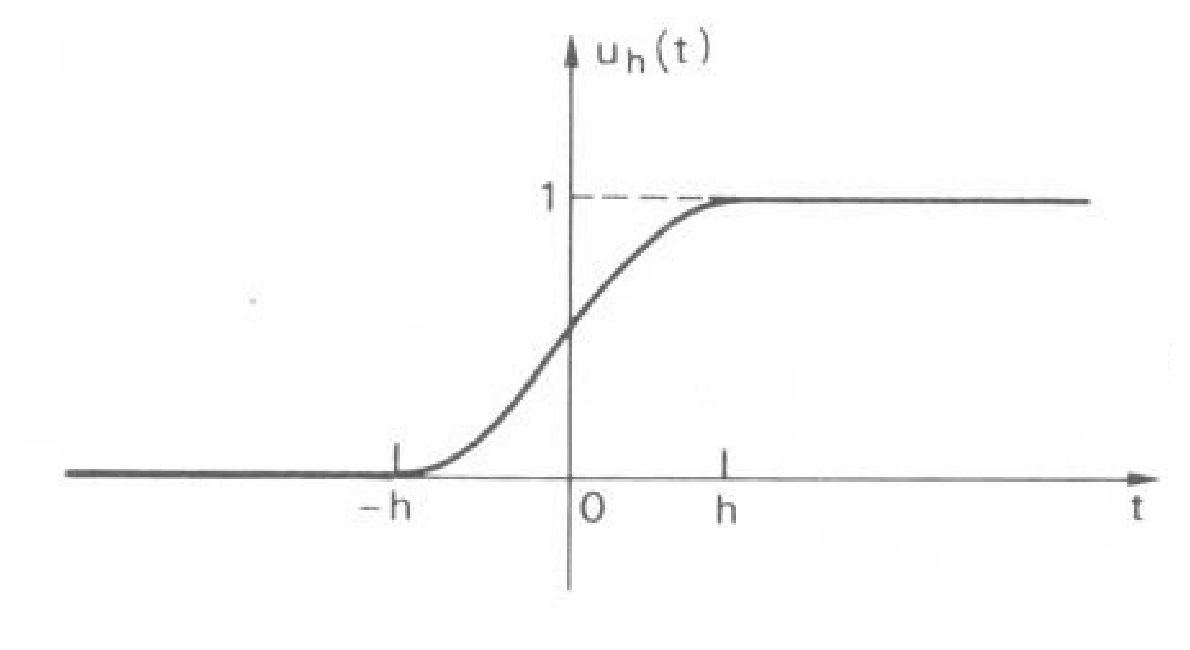
\includegraphics[width=6cm]{imatges/esglaoreal.eps} & &
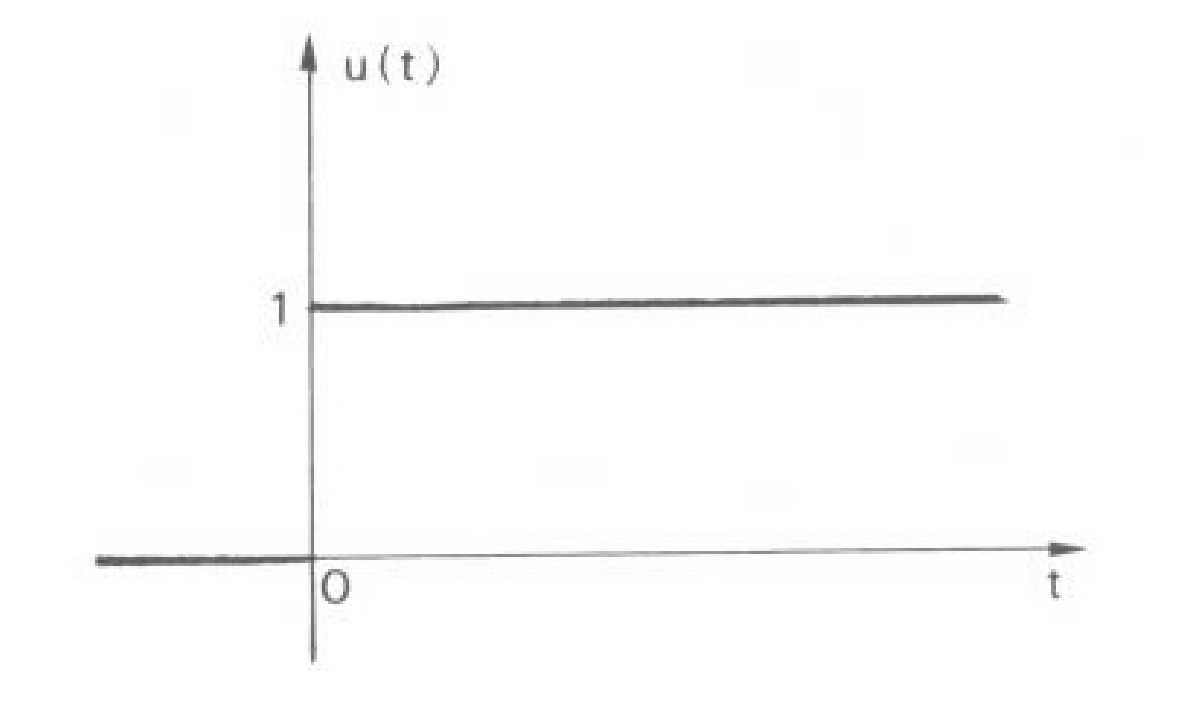
\includegraphics[width=6cm]{imatges/esglaoideal.eps}
\end{tabular}
\caption{[Gasquet-Witomski]. Esquerra, funci\'o esgla\'o real. 
Dreta, idealitzaci\'o de la funci\'o anterior (funci\'o esgla\'o unitari o
de Heaviside).}
\label{esglao.fig}
\end{figure}

\begin{figure}[htbp]
\begin{tabular}{lcr}
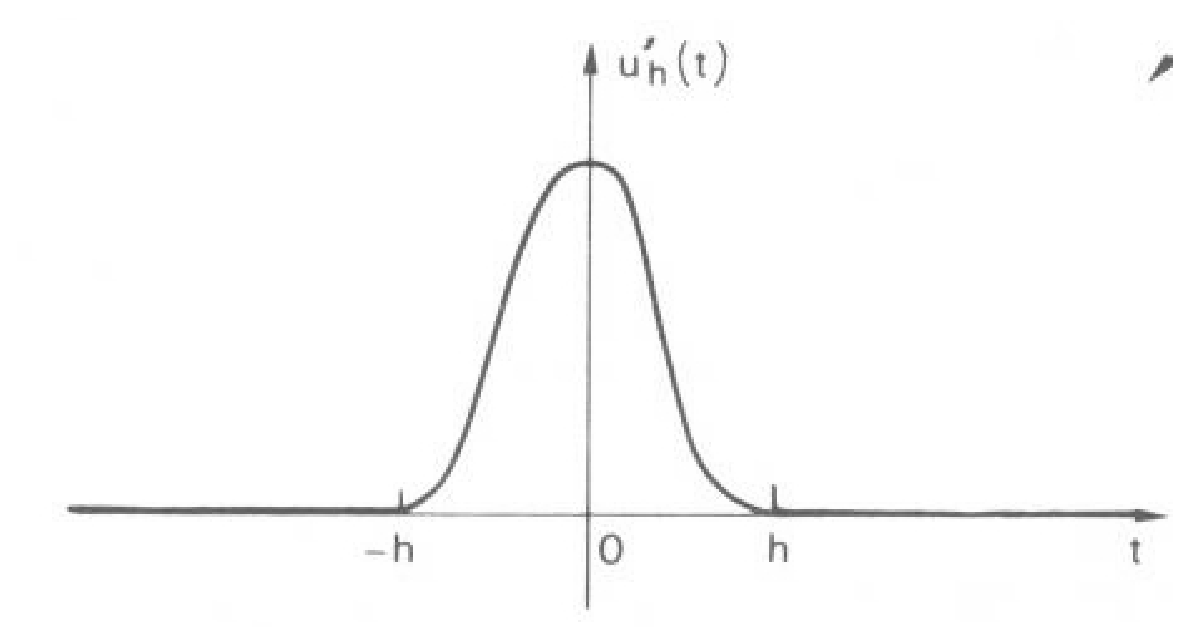
\includegraphics[width=4cm]{imatges/deltareal.eps} & 
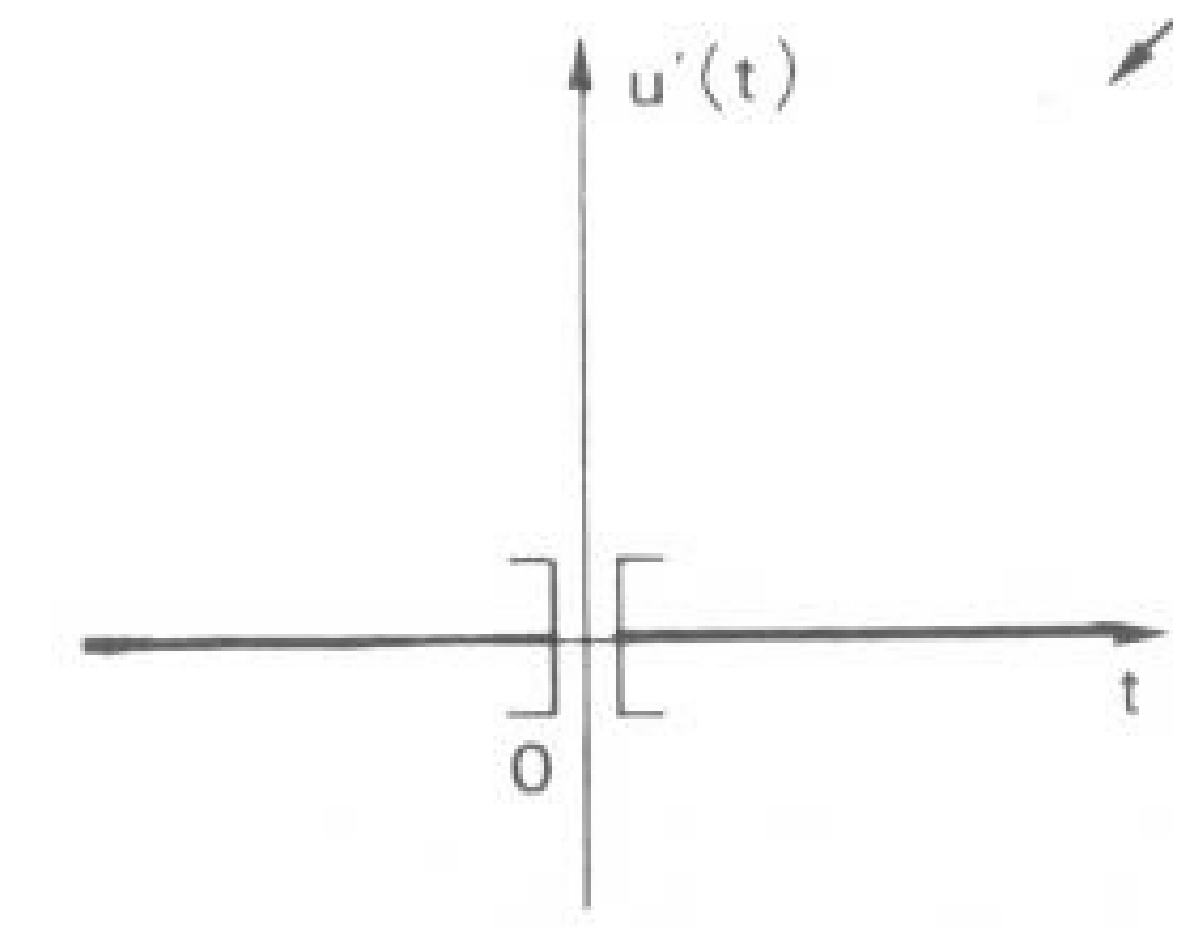
\includegraphics[width=4cm]{imatges/deltamatematic.eps} & 
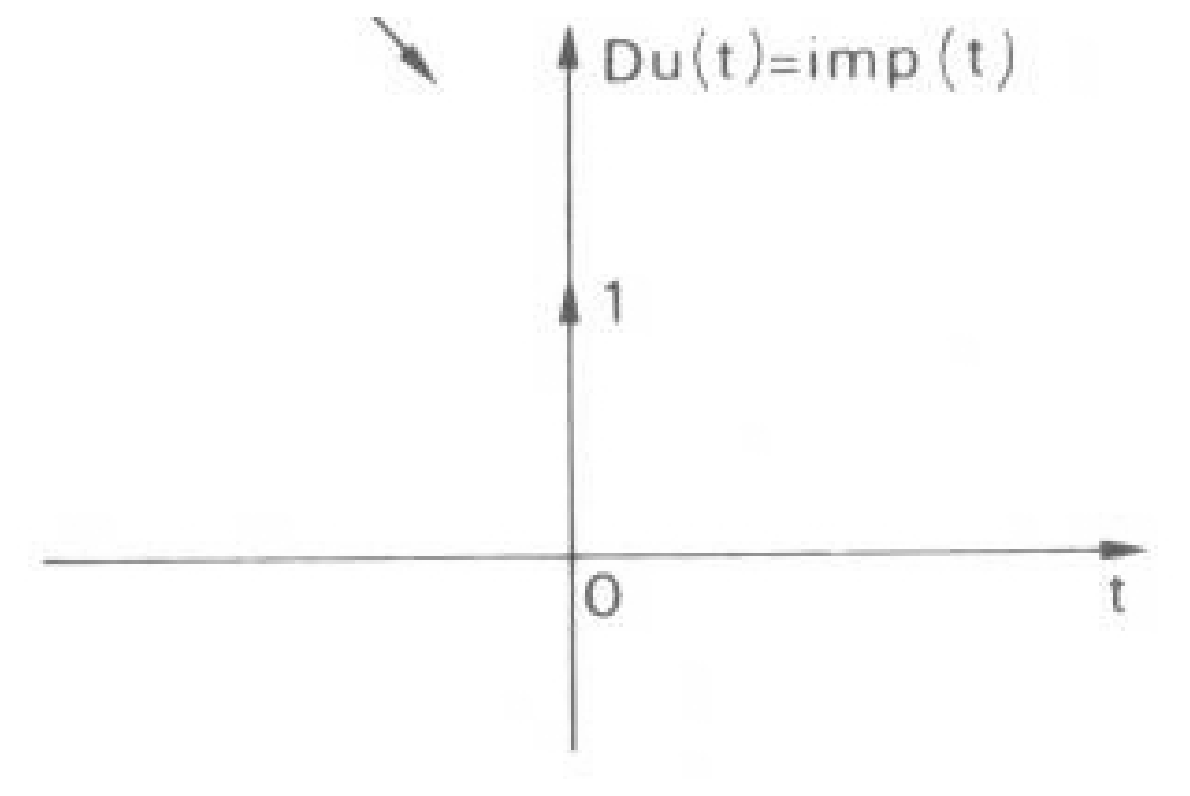
\includegraphics[width=4cm]{imatges/deltaideal.eps}
\end{tabular}
\caption{[Gasquet-Witomski]. Esquerra, derivada d'una funci\'o esgla\'o real. 
Centre, derivada de la funci\'o esgla\'o ideal.
Dreta, idealitzaci\'o de la derivada de l'esgla\'o real
(delta de Dirac o impulsi\'o).}
\label{delta.fig}
\end{figure}


\vskip 0.2 cm 
La propietat $\int_{-\infty}^{+\infty} \delta(x) dx = 1$
 contradiu la definici\'o d'integral utilitzada
pels matem\`atics (la integral de Lebesgue de $\delta(x)$ \'es nula), per 
tant la ``funci\'o'' $\delta$ no t\'e sentit des d'un punt de vista
matem\`atic, malgrat la seva gran utilitat pr\`actica. 
V\`aren haver de passar 20 anys fins que els matem\`atics (especialment 
L. Schwartz i S.L. Sobolev) don\`assin sentit a la $\delta$ de Dirac, en 
el marc d'una teoria m\'es \`amplia anomenada 
{\bf Teoria de les Distribucions}.   
Actualment les distribucions s\'on indispensables en l'an\`alisi 
matem\`atica i les matem\`atiques aplicades. 

\vskip 0.3 cm
\textbf{Definici\'o}. Sigui ${\cal D}$ l'espai de les funcions 
${\cal C}^\infty$ que s'anul.len f\'ora d'un cert interval (${\cal D}$ \'es
conegut com l'{\bf espai de les funcions test o prova}). 
Una {\bf distribuci\'o} $T$ \'es una transformaci\'o lineal i cont\'\i nua 
$T:{\cal D} \rightarrow \C$.
La continuitat de $T$ significa que si $\varphi_n \rightarrow \varphi$ uniformement
en conjunts afitats, totes les derivades de $\varphi_n$ convergeixen 
uniformement a les derivades de $\varphi$ en conjunts afitats i totes les 
funcions $\varphi_n$ s'anul.len fora d'un conjunt compacte fixe, llavors
$T(\varphi_n) \rightarrow T(\varphi)$.

\vskip 0.2 cm
La variable d'una distribuci\'o \'es per tant una funci\'o test i el seu 
valor una nombre complexe. La valor de $T$ en $\varphi$ es denotar\`a 
de manera indiferent com a $T(\varphi)$ o $\langle T, \varphi \rangle$.

\vskip 0.3 cm
\noindent
\textbf{Exemples}.
\begin{enumerate}[Exemple 1.]
\item Distribuci\'o delta de Dirac.
Donat un nombre real $a$ definim l'aplicaci\'o 
$\delta_a : {\cal D} \rightarrow \C$ com $\delta_a(\varphi)=\varphi(a)$.
Es pot demostrar que aquesta \'es una aplicaci\'o lineal i cont\'\i nua.
Per a $a=0$ la denotam simplement com $\delta$.
\newline
Podem observar com hem definit la distribuci\'o delta a partir d'una
de les seves propietats: la que defineix la seva interacci\'o amb altres 
funcions.
\item Pinta de Dirac. Aquesta distribuci\'o es denota com 
$T=\Delta_a=\sum_{-\infty}^{+\infty} \delta_{na}$
i es defineix de la seg\"uent manera: 
\[
\forall \varphi \in {\cal D} \qquad \qquad T(\varphi)=
\sum_{-\infty}^{+\infty} \varphi(na)
\] 
\end{enumerate}

\vskip 0.3 cm
\noindent
\textbf{Les distribucions com a funcions generalitzades}. La majoria
de les funcions es poden considerar com distribucions mitjan\c{c}ant
la identificaci\'o que resulta del seg\"uent teorema:
\newline
\noindent
\textbf{Teorema}. Si $f$ \'es una funci\'o localment integrable 
($f \in L^1_{\mathrm{loc}}(\R)$), llavors l'aplicaci\'o 
$T_f:{\cal D} \rightarrow \C$ definida com
\begin{equation}
\label{defDist}
T_f(\varphi)=\int_{-\infty}^{+\infty} f(x) \varphi(x) dx
\end{equation}
\noindent
\'es una distribuci\'o.

\vskip 0.2 cm
El teorema precedent implica que a qualsevol funci\'o de 
$L^1_{\mathrm{loc}}(\R)$ li podem assignar una distribuci\'o. A m\'es,
\'es possible demostrar que aquesta assignaci\'o \'es \'unica:
\begin{equation}
T_f = T_g  \quad  \Longleftrightarrow \quad f=g \qquad \mathrm{g.p.t}
\end{equation}
 
\noindent
De manera que podem identificar $f$ amb la seva distribuci\'o associada.

\vskip 0.3 cm
\noindent
\textbf{Derivaci\'o de distribucions}. Aquesta definici\'o ha d'\'esser
consistent amb la definici\'o de derivada d'una funci\'o, tenint en
compte que una distribuci\'o es pot considerar com una generalitzaci\'o
del concepte de funci\'o.
Una manera de generalitzar la definici\'o de derivada \'es a partir
de l'equaci\'o (\ref{defDist}) i la f\`ormula de la derivaci\'o per parts:
\begin{equation}
\label{eqDeriv}
\begin{array}{lcl}
\langle T_{f'}, \varphi \rangle & = & 
\int_{-\infty}^{+\infty} f'(x) \varphi(x) dx =
\{
\begin{array}{lcl}
du=f'(x) dx & \rightarrow & u=f(x)\\
v=\varphi(x)   & \rightarrow & dv=\varphi'(x) dx
\end{array}
\} = \\
\\
   & = &
(f(x) \varphi(x) ]_{-\infty}^{+\infty} -
\int_{-\infty}^{+\infty} f(x) \varphi'(x) dx=
- \int_{-\infty}^{+\infty} f(x) \varphi'(x) dx= \\
\\
   & = & - \langle T_f, \varphi' \rangle
\end{array}
\end{equation}
\noindent
la pen\'ultima igualtat \'es deguda a que $\varphi(x)$ t\'e suport afitat
i per tant $\varphi(-\infty)=\varphi(+\infty)=0$.
\newline
En general s'ext\'en aquesta definici\'o per a qualsevol distribuci\'o
diguent que la derivada $T'$ de la distribuci\'o $T$ cumpleix:
\[
\forall \varphi \in {\cal D} \qquad \langle T', \varphi \rangle = 
- \langle T, \varphi' \rangle
\]

\vskip 0.2 cm
\noindent
\textbf{Exemples}.
\begin{enumerate}[Exemple 1.]
\item Derivada de $\delta_a$. 
\[
\delta'_a(\varphi)=\langle \delta'_a, \varphi \rangle=
-\langle \delta_a, \varphi' \rangle = -\varphi'(a)
\]
\item Derivada de l'esgla\'o unitari. Recordem que 
\[
u(t)=\begin{cases}
1 & \mathrm{si} \qquad t >=0\\
0 & \mathrm{resta}
\end{cases}
\]
\noindent
llavors 
\[
\begin{array}{lcl}
\langle T'_u, \varphi \rangle & = & -\langle T_u, \varphi' \rangle =
-\int_0^{+\infty} \varphi'(x) dx=\\
\\
 & = & -(\varphi(+\infty)-\varphi(0))=-(0-\varphi(0))=
\varphi(0)=\langle \delta, \varphi \rangle 
\end{array}
\]
\noindent
per tant la derivada de la funci\'o esgla\'o unitari \'es la $\delta$ de 
Dirac, la qual cosa coincideix amb la noci\'o intuitiva de $\delta(x)$ 
que s'ha comentat al comen\c{c}ament d'aquesta secci\'o.
\end{enumerate}

\vskip 0.2 cm
\noindent
\textbf{Derivaci\'o de funcions amb discontinu\"\i tats}. L'expressi\'o
per a la derivada d'una distribuci\'o dedu\"\i da en (\ref{eqDeriv})
nom\'es t\'e sentit si $f'(x)$ est\'a definida per a tots els valors de
$\R$. Per a una funci\'o $f$ discont\'\i nua la $f'(x)$ no est\'a 
definida en els punts de discontinu\"\i tat. No obstant, si la funci\'o 
\'es derivable entre els punts de discontinu\"\i tat i en aquests punts 
el l\'\i mit de la funci\'o a esquerra i a dreta \'es finit, la derivada 
en el sentit de les distribucions es pot calcular.
\newline
Considerem una funci\'o cont\'\i nuament derivable en els intervals 
$(-\infty, a)$, $(a, b)$ i $(b, +\infty)$, amb l\'\i mits laterals 
seg\"uents en els punts de discontinu\"\i tat: $f(a-)$, $f(a+)$,
$f(b-)$, $f(b+)$. Llavors la derivada en el sentit de les distribucions
de $f$ \'es
\[
T'_f = T_{f'} + (f(a+)-(f(a-)) \delta_a + (f(b+)-f(b-)) \delta_b
\]

\begin{figure}[htbp]
\begin{center}
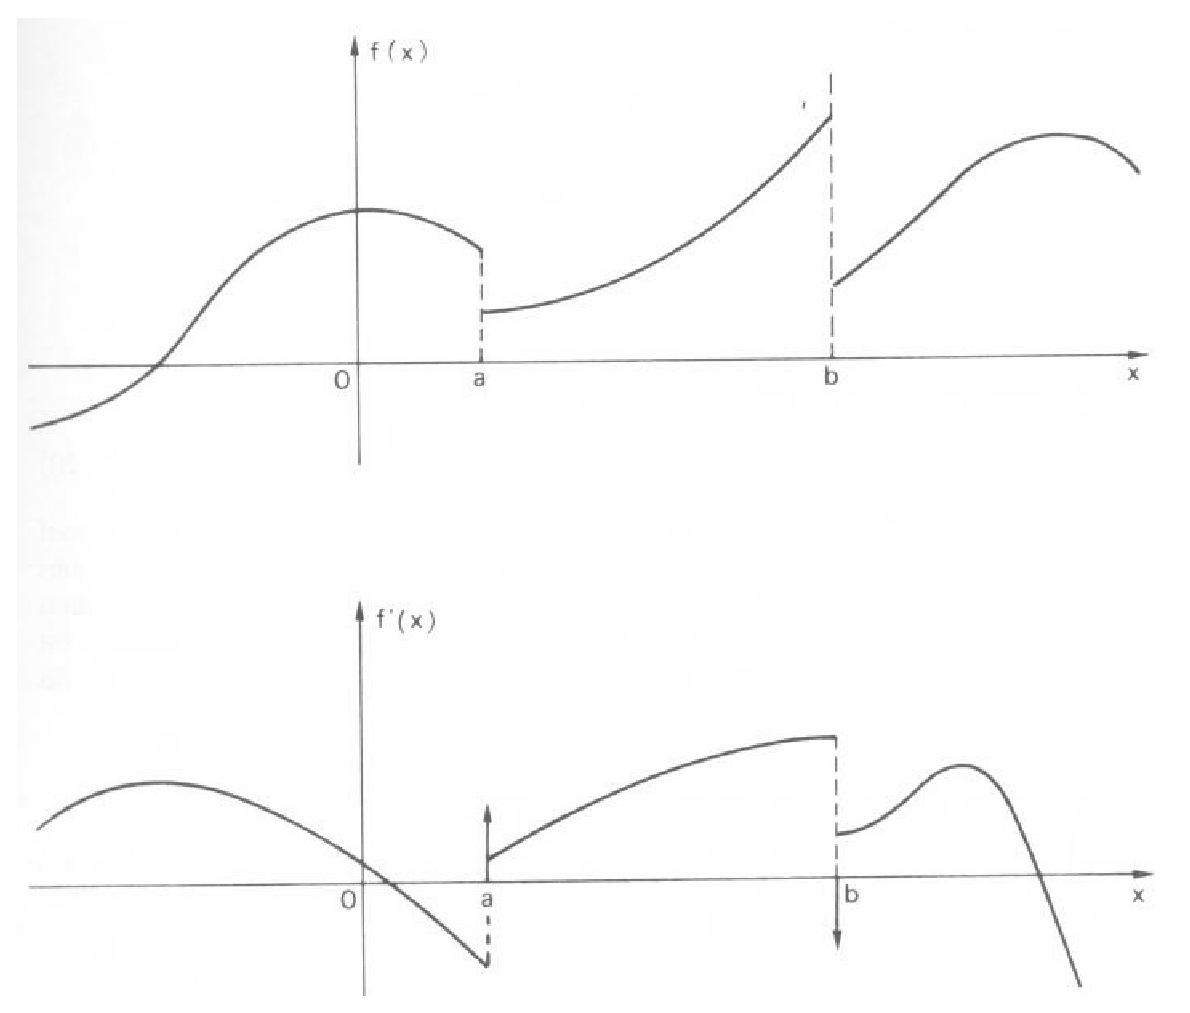
\includegraphics[width=10cm]{imatges/derdiscontinua.eps}
\caption{Derivada, en el sentit de les distribucions d'una funci\'o
discont\'\i nua.}
\label{derBot.fig}
\end{center}
\end{figure}

\noindent
En general, per a un nombre $m$ de discontinuitats apareixeran $m$ 
distribucions puntuals $\delta$ situades en els punts de discontin\"\i tat
i afectades per un coeficient igual a la magnitud del bot de 
discontinu\"\i tat.

\noindent
\textbf{Exemple}. La derivada en el sentit de les distribucions de la funci\'o 
peri\`odica definida en $(0, a)$ $f(x)=\frac{x}{a}$ \'es 
$f'=\frac{1}{a} - \sum_{n=-\infty}^{+\infty} \delta_{na}$

\vskip 0.2 cm
\noindent
\textbf{Teorema. Derivada terme a terme d'una s\`erie}. Sigui 
$((u_n(x))_{n \in \N}$ una successi\'o de funcions absolutament cont\'\i nues
sobre tot interval afitat tal que la s\`erie 
$\sum_{n=0}^{+\infty} u_n(x)$ convergeix en el sentit de les distribucions
cap a una funci\'o $f$ localment integrable. Llavors la s\`erie derivada 
$\sum_{n=0}^{+\infty} u'_n(x)$ convergeix en el sentit de les distribucions
cap a la derivada $f'$ de $f$.

\vskip 0.3 cm
\noindent
\textbf{Propietat}. Direm que dues distribucions $T_1$ i $T_2$ s\'on iguals si
$\forall \varphi \in {\cal D}$, 
$\langle T_1, \varphi \rangle = \langle T_2, \varphi \rangle$.

\vskip 0.3 cm 
\noindent
La seg\"uent expressi\'o s'emplear\`a m\'es endavant en aquest tema.
\newline
\noindent
\textbf{F\`ormula de Poisson}. 
\begin{equation}
\label{Poisson}
\sum_{n=-\infty}^{+\infty} \delta(t-na)=
\frac{1}{a} \sum_{n=-\infty}^{+\infty} e^{i 2 \pi n \frac{x}{a}}
\end{equation}

\vskip 0.3 cm
\noindent
\textbf{Transformada de Fourier de distribucions}.
Seguint el mateix raonament que ens ha perm\'es trobar una expressi\'o 
per a la derivada d'una distribuci\'o compatible amb la noci\'o habitual
de derivada, ara volem trobar una expressi\'o per a la transformada de 
Fourier d'una distribuci\'o compatible amb la definici\'o 
cl\`assica. Novament partim de l'equaci\'o (\ref{defDist}) 
i en aquest cas aplicam el 
Teorema de Fubini:
\[
\begin{array}{lcl}
\langle \hat{f} , \varphi \rangle & = &
\int_{-\infty}^{+\infty} (\int_{-\infty}^{+\infty} e^{- i 2 \pi \xi x} 
f(x) dx ) \varphi(x) d\xi \\
\\
 & = & \int_{-\infty}^{+\infty} f(x) 
\int_{-\infty}^{+\infty} e^{- i 2 \pi \xi x} \varphi(x) d\xi dx= \\
\\
 & = & \int_{-\infty}^{+\infty} f(x) \hat{\varphi}(x) dx = 
\langle f, \hat{\varphi} \rangle
\end{array}
\]

\noindent
per tant
\begin{equation}
\label{FTransform}
\langle \hat{T}, \varphi \rangle = \langle T, \hat{\varphi} \rangle
\end{equation}

\vskip 0.2 cm
Evidentment el raonament anterior no t\'e sentit si $\hat{\varphi}$ no pertany a
l'espai de les funcions test. El problema \'es que si $\varphi \in {\cal D}$
llavors $\hat{\varphi}$ no estar\`a dins ${\cal D}$. Aix\'o ens porta a
considerar un nou espai de funcions test, denotat ${\cal S}(\R)$ i que
representa les funcions amb decreixement r\`apid
(una funci\'o $f$ \'es de decreixement r\`apid si $\forall p \in \N$ 
$\lim_{|x| \rightarrow \infty} |x^p f(x) | = 0$). 
Aquest espai de funcions
\'es estable per transformacions de Fourier i
ens defineix un nou tipus de distribucions anomenades {\bf distribucions
temperades}. Les distribucions temperades formen un subespai de l'espai
de distribucions habituals. L'equaci\'o (\ref{FTransform}) t\'e sentit
quan ens referim a les distribucions temperades.

\vskip 0.2 cm
\noindent
\textbf{Exemples}.
\begin{enumerate}[Exemple 1.]
\item Delta de Dirac. 
\[
\langle \hat{\delta}, \varphi \rangle = \langle \delta, \hat{\varphi} \rangle =
\hat{\varphi}(0)=\int_{-\infty}^{+\infty} \varphi(x) dx = 
\langle 1, \varphi \rangle
\]
\noindent
De la mateixa manera
\[
\langle \hat{\delta_a}, \varphi \rangle = 
\langle \delta_a, \hat{\varphi} \rangle =
\int_{-\infty}^{+\infty} e^{- i 2 \pi a \lambda} \varphi(\lambda) d\lambda
\]
\noindent
i per tant $\hat{\delta_a}(\xi)=e^{- i 2 \pi a \xi}$.
\item Pinta de Dirac.
\[
\widehat{\Delta_a}=\sum_{n=-\infty}^{+\infty} \widehat{\delta_{na}} =
\sum_{n=-\infty}^{+\infty} e^{-i 2 \pi n a \xi} = 
\frac{1}{a} \sum_{n=-\infty}^{+\infty} \delta_{\frac{n}{a}} =
\frac{1}{a} \Delta_{\frac{1}{a}}
\]
\noindent
la darrera igualtat s'obt\'e a partir de la f\`ormula de Poisson.
\end{enumerate}

\vskip 0.5 cm
\noindent
\textbf{Utilitzaci\'o pr\`actica de la distribuci\'o delta}.
De la mateixa manera que a una funci\'o $f$ li assignam la distribuci\'o
$T_f$ definida per l'equaci\'o (\ref{defDist}), en la pr\`actica associam
la distribuci\'o $\delta$ a una ``funci\'o'' $\delta(t)$ tal que 
\[
\int_{-\infty}^{+\infty} \delta(t) \varphi(t) dt = \varphi(0) \qquad 
\forall \varphi \in {\cal D}
\]
\noindent 
Aquesta $\delta(t)$ \'es la cl\`assica delta de Dirac.

De manera an\`aloga, la distribuci\'o pinta de Dirac $\Delta_a$ s'associa
a la ``funci\'o'' 
\[
\Delta_a(t)=\sum_{n=-\infty}^{+\infty} \delta(t-na)
\]

En els c\`alculs que desenvoluparem en els seg\"uents apartats
treballarem amb aquestes ``funcions''.

\vskip 0.5 cm
Arribats a aquest punt ja disposam de totes les eines necess\`aries 
per estudiar, des d'un punt de vista matem\`atic, el proc\'es de
discretitzaci\'o.
\subsection{Mostreig de funcions. Teorema de Shannon.}
\label{mostreig}
\subsubsection{Representaci\'o de funcions discretes.}
Com ja s'ha comentat al principi d'aquesta secci\'o una manera de 
descriure una funci\'o discreta \'es mitjan\c{c}ant la notaci\'o
\[
f[n]=f(nT), \qquad n \in \Z
\]
\noindent
on f(t) \'es la funci\'o cont\'\i nua original i $T$ el per\'\i ode de
mostreig.

No obstant aquesta representaci\'o no \'es \'util si volem, per exemple,
calcular la transformada de Fourier de la funci\'o discreta. En aquest cas
\'es necessari dispossar d'una representaci\'o en funci\'o de la variable
$t$. Una possibilitat \'es definir la versi\'o discreta de $f(t)$ com
\[
f_d(t)=\begin{cases}
f(nT) & \mathrm{si} \qquad t=nT, \quad n \in \Z\\
0    & \mathrm{resta}
\end{cases}
\]

El problema d'aquesta representaci\'o \'es que $f_d(t)$ nom\'es pren
valors no nuls en un conjunt discret de punts, els quals tenen mesura
zero i per tant qualsevol calcul integral que intentem (per exemple
una transformada de Fourier) valdr\`a zero.

Una manera d'evitar aquest inconvenient \'es definint $f_d$ com una
distribuci\'o. En particular, definim $f_d$ com la distribuci\'o
que t\'e associada la ``funci\'o''
\begin{equation}
\label{sampledf}
f_d(t)=\sum_{n=-\infty}^{+\infty} f(nT) \delta(t-nT)
\end{equation}

Gr\`aficament aquesta funci\'o \'es representa com en la Figura 
\ref{sampled.fig}.

\begin{figure}[htbp]
\begin{tabular}{lcr}
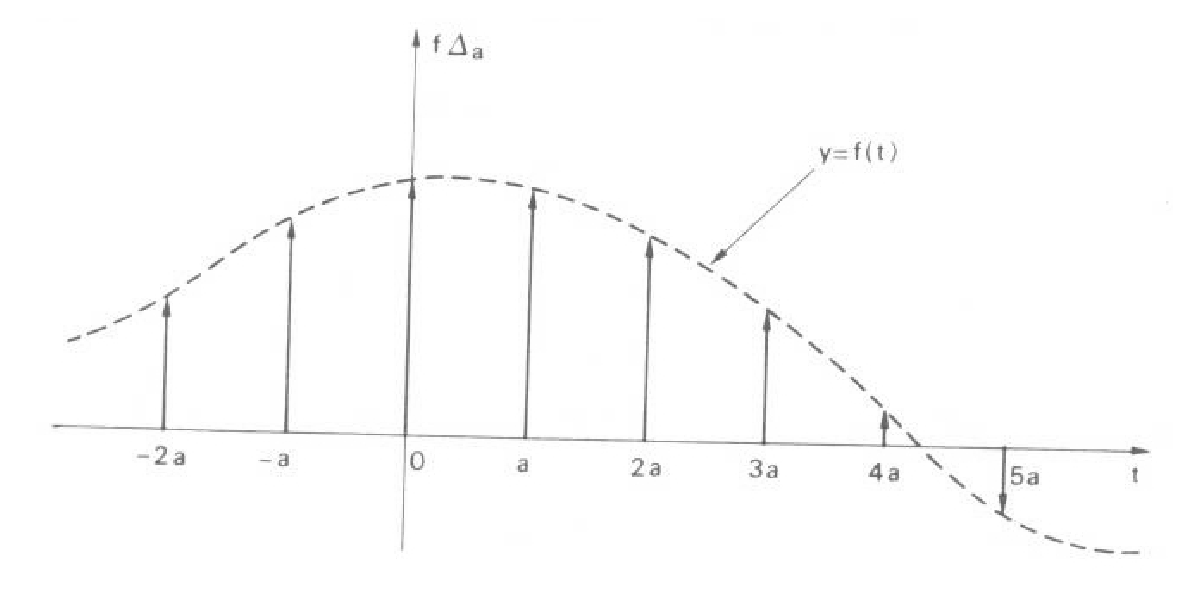
\includegraphics[width=6cm]{imatges/sampledf.eps} & &
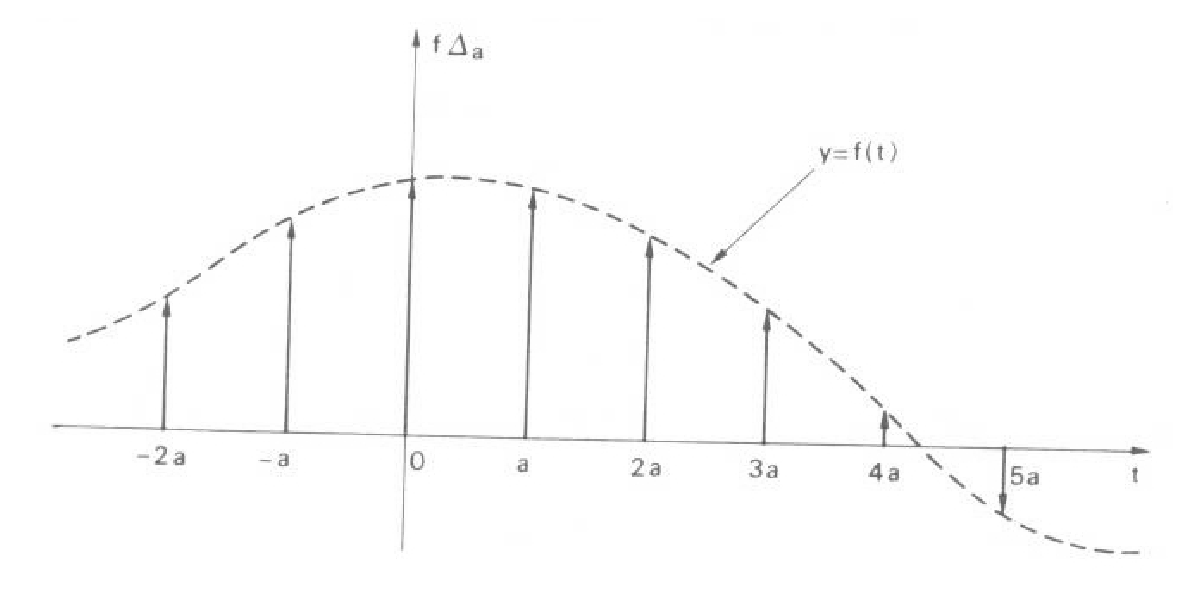
\includegraphics[width=6cm]{imatges/sampledf.eps}
\end{tabular}
\caption{[Oppenheim] Esquerra, funci\'o mostrejada amb
una pinta de Dirac o tren d'impulsos. Dreta, funci\'o discreta.}
\label{sampled.fig}
\end{figure}

Com que $f_d$ \'es una distribuci\'o i s'escriu com una suma ponderada de
deltes, podrem calcular la seva transformada de Fourier aplicant els resultats
que hem vist a la secci\'o anterior:

\begin{equation}
\label{sampledFT}
\hat{f}_d(\xi)=\sum_{n=-\infty}^{+\infty} f(nT) \widehat{\delta(t-nT)}(\xi)=
\sum_{n=-\infty}^{+\infty} f(nT) e^{- i 2 \pi n T \xi}
\end{equation}

\vskip 0.3 cm
\'Es possible arribar a aquest resultat raonant d'una altra manera i sense
rec\`orrer a la teoria de les distribucions.
\newline
Consideram una funci\'o $\tilde{f}_d(t)$ que aproxima la funci\'o 
discretitzada.
\[
\tilde{f}_d(t)=\sum_{n=-\infty}^{+\infty} f(nT) D_\epsilon(t-nT)
\]
\vskip 0.1 cm
\noindent
on $D_\epsilon(t)=\frac{1}{\epsilon} {\cal X}_{[-\epsilon, +\epsilon]}$.
Podem considerar aquesta funci\'o com una aproximaci\'o de la funci\'o
$\delta(t)$. A m\'es $\int_\R D_\epsilon (t) dt = 1$.

\begin{figure}[htbp]
\begin{center}
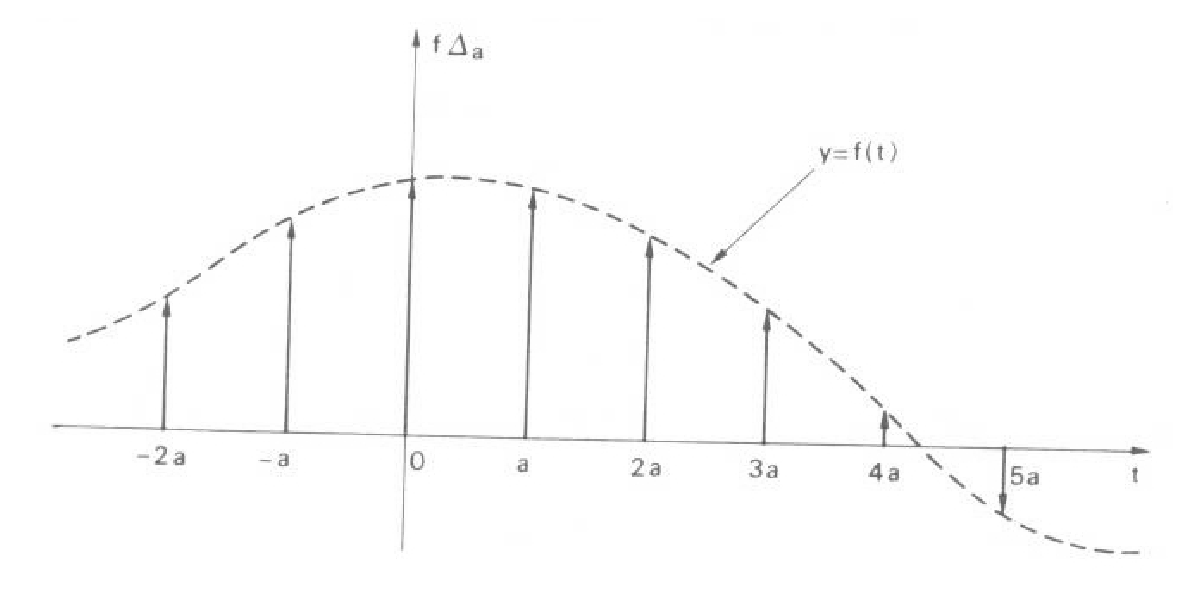
\includegraphics[width=9cm]{imatges/sampledf.eps}
\caption{Representaci\'o aproximada d'una funci\'o discreta}
\end{center}
\end{figure}

Definida d'aquesta manera la funci\'o $\tilde{f}(t)$ pren els valors
\[
\tilde{f}_d(t)=\begin{cases}
\frac{1}{\epsilon} f(nT) & \mathrm{si} 
\qquad t \in [nT-\frac{\epsilon}{2}, nT+\frac{\epsilon}{2}], 
\quad n \in \Z\\
0    & \mathrm{resta}
\end{cases}
\]

\vskip 0.1 cm
Si calculam la transformada de Fourier d'aquesta funci\'o obtenim
el seg\"uent resultat
\[
\begin{array}{lcl}
\hat{\tilde{f}}_d(\xi) & = & \int_{-\infty}^{+\infty} \tilde{f}(t) 
e^{- i 2 \pi \xi t} dt=\sum_{n=-\infty}^{+\infty} \frac{1}{\epsilon} f(nT) 
\int_{nT-\frac{\epsilon}{2}}^{nT+\frac{\epsilon}{2}} e^{- i 2 \pi \xi t} dt\\
\\
 & = &
\sum_{n=-\infty}^{+\infty} f(nT) e^{-i 2 \pi \xi n T}
\frac{\sin(\pi \xi \epsilon)}{\pi \xi \epsilon}
\end{array}
\]

Si ara fem $\epsilon$ tendir cap a zero $\tilde{f}_d$ tendeix cap a $f_d$
i la seva transformada tendeix cap a $\hat{f}_d$

\[
\hat{f}_d(\xi)=\lim_{\epsilon \rightarrow 0} \hat{\tilde{f}}_d(\xi)=
\sum_{n=-\infty}^{+\infty} f(nT) e^{-i 2 \pi \xi n T} 
(\lim_{\epsilon \rightarrow 0} \frac{\sin(\pi \xi \epsilon)}{\pi \xi \epsilon})
=\sum_{n=-\infty}^{+\infty} f(nT) e^{-i 2 \pi \xi n T}
\]
\noindent
on el l\'\i mit s'ha calculat utilitzant la regla de l'H\^opital.

\vskip 0.1 cm
Podem observar com aquesta \'es la mateixa expressi\'o a la qual
arrib\`avem emprant en raonament bassat en les deltes de Dirac.

\vskip 0.6 cm
La seg\"uent proposici\'o relaciona les transformades de Fourier de $f_d$
i $f$.

\vskip 0.2 cm
\noindent
\textbf{Proposici\'o}. La transformada de Fourier d'un senyal discret
$f_d$ obtingut per mostreig de $f$ a intervals $T$ val
\begin{equation}
\label{samplingtheorem}
\hat{f}_d(\xi)=\frac{1}{T} \sum_{n=-\infty}^{+\infty} \hat{f} (\xi - 
\frac{n}{T})
\end{equation}

\noindent
\underline{Dem}. Com que $\delta(t-nT)$ \'es nul fora de $t=nT$
podem dir que 
\[
f(nT) \delta(t-nT) = f(t) \delta(t-nT)
\]
\noindent
de manera que podem reescriure l'expressi\'o (\ref{sampledf}) com
\[
f_d(t)=\sum_{n=-\infty}^{+\infty} f(t) \delta(t-nT)=
f(t) \sum_{n=-\infty}^{+\infty} \delta(t-nT)=f(t) \Delta_T(t)
\]

\noindent
La transformada de Fourier de $f_d(t)$ ser\`a per tant
\[
\begin{array}{lcl}
\hat{f}_d(\xi) & = &\hat{f}(\xi) * \widehat{\Delta_T}(\xi)=
\hat{f}(\xi) * \frac{1}{T} \Delta_{\frac{1}{T}}(\xi) = \\ \\ & = & 
\frac{1}{T} \hat{f}(\xi) * \sum_{n=-\infty}^{+\infty} \delta(\xi-\frac{n}{T})=
\frac{1}{T} \sum_{n=-\infty}^{+\infty} \hat{f}(\xi) * \delta(\xi-\frac{n}{T})=
\\ \\ & = &
\frac{1}{T} \sum_{n=-\infty}^{+\infty} \hat{f}(\xi-\frac{n}{T})
\end{array}
\]
\begin{flushright}
$\square$
\end{flushright}

\vskip 0.3 cm
La proposici\'o anterior mostra que el mostreig de $f$ a intervals $T$
fa la seva transformada de Fourier $\frac{1}{T}$-peri\`odica, degut a la
suma de les versions translladades $\hat{f}(\xi-\frac{n}{T})$.
La seg\"uent figura mostra un exemple de la transformada de Fourier 
d'una funci\'o i de la seva versi\'o discreta.  

\skip 0.1 cm

\begin{figure}[htbp]
\begin{center}
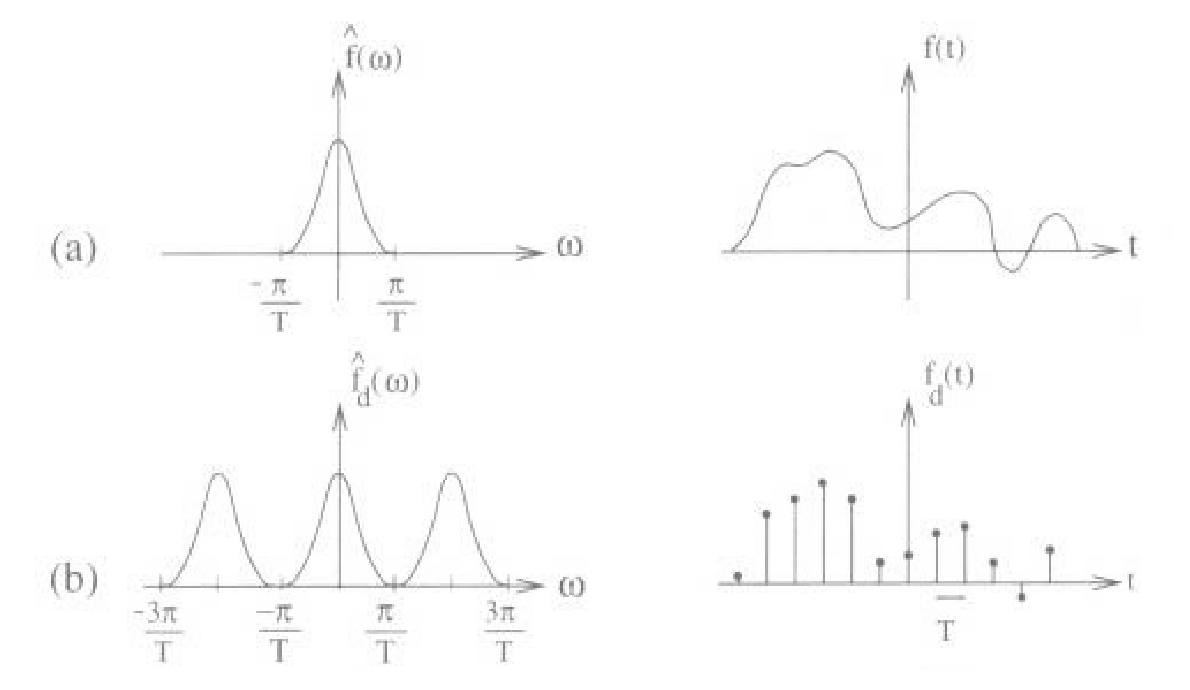
\includegraphics[width=10cm]{imatges/samplingtheorem.eps}
\caption{
%\cite{Mallat}.
[Mallat].
(a) Senyal $f$ i la seva Transformada de Fourier 
$\hat{f}$.(b) Un mostreig uniforme de $f$ fa la seva transformada de Fourier
peri\`odica.}
\label{samplingFT.fig}
\end{center}
\end{figure}

\vskip 0.3 cm
\subsubsection{Reconstrucci\'o d'un senyal continu a partir de les
seves mostres. Teorema de mostreig.}
El seg\"uent teorema ens diu quines condicions s'han de cumplir per
poder reconstruir un senyal continu a partir de les seves mostres
i tamb\'e ens d\'ona una f\`ormula per a la reconstrucci\'o.
\newline
\noindent
\textbf{Teorema de mostreig (Shannon-Whitaker).} Si el suport de $\hat{f}$
est\`a incl\'os dins $[-\frac{1}{2T}, +\frac{1}{2T}]$ llavors
\begin{equation}
\label{shannonTh}
f(t)=\sum_{n=-\infty}^{+\infty} f(nT) h_T(t-nT)
\end{equation}
\noindent
on
\[
h_T(t)=\frac{\sin(\pi t / T)}{\pi t / T}
\]

\vskip 0.1 cm
\noindent
\underline{Dem}. Com que $\hat{f}(\xi)=0$ quan $|\xi| > \frac{1}{2T}$
el suport de $\hat{f}(\xi)$ i el de $\hat{f}(\xi-\frac{n}{T})$ tenen
intersecci\'o nul.la per a $n \neq 0$, per tant
\begin{equation}
\label{supfd}
\hat{f}_d(\xi)=\frac{\hat{f}(\xi)}{T} \qquad \mathrm{si} \qquad 
|\xi| < \frac{1}{2T}  
\end{equation}

\noindent
Com el suport de $\hat{f}$ est\`a dins $[-\frac{1}{2T}, \frac{1}{2T}]$
podem escriure que

\[
\hat{f}(\xi)=\begin{cases}
T \hat{f}_d(\xi) & \mathrm{si} \qquad |\xi| < \frac{1}{2T}  \\
0 & \mathrm{resta}
\end{cases} \qquad = T \hat{f}_d(\xi) {\cal X}_{[-\frac{1}{2T}, \frac{1}{2T}]}
\] 

\noindent
Ara b\'e, la transformada de Fourier de $h_T$ val 
$T {\cal X}_{[-\frac{1}{2T}, \frac{1}{2T}]}$ per tant
\[
\hat{f}(\xi)=\hat{f}_d(\xi) \hat{h}_T(\xi)
\] 
\noindent
i en conseq\"u\`encia (emprant la igualtat (\ref{sampledf}))
\[
\begin{array}{lcl}
f(t) = f_d(t) * h_T(t) &  = & 
h_T(t) * \sum_{n=-\infty}^{+\infty} f(nT) \delta(t-nT) =\\ \\
 & = & \sum_{n=-\infty}^{+\infty} f(nT) (h_T(t) * \delta(t-nT)) = \\ \\
 & = & \sum_{n=-\infty}^{+\infty} f(nT) h_T(t-nT)  
\end{array}
\]
\begin{flushright}
$\square$
\end{flushright}

\vskip 0.3 cm
La condici\'o de que el suport de $\hat{f}$ estigui limitat a un
cert rang de freq\"u\`encies s'interpreta intuitivament com una
exig\`encia a la funci\'o $f$ perqu\`e no varii de manera brusca
entre dues mostres consecutives, de manera que la interpol.laci\'o
entre els valors de les mostres sigui possible.

\vskip 0.2 cm
El valor $\frac{1}{2T}$, que defineix el suport m\`axim
de $\hat{f}$ que assegura la reconstrucci\'o de $f$, reb el nom de 
{\bf freq\"u\`encia de Nyquist}.

\subsubsection{Aliasing}
Fins ara hem considerat el problema del mostreig des del
punt de vista de les condicions que ha de cumplir el senyal
mostrejat per poder reconstruir el senyal original a partir
de les mostres. Un plantejament diferent del problema \'es 
considerar que el senyal continu ens ve donat i volem
saber quina \'es la millor manera de mostrejar-lo. Aix\'o
equival a trobar el valor de $T$ que ens permet tenir el 
m\'\i nim nombre de mostres a partir de les quals reconstruir
el senyal original.
\newline
En primer lloc \'es evident que el nombre de mostres ser\`a m\'es 
petit com major sigui $T$. Per altra banda,
si el suport freq\"uencial del senyal continu es troba
en l'interval $[-\xi_{\mathrm{max}}, +\xi_{\mathrm{max}}]$, 
s'haur\`a de cumplir que $\frac{1}{2T} \geq \xi_{\mathrm{max}}$.
Per tant el valor \`optim del per\'\i ode de mostreig \'es 
$T_{\mathrm{max}} = \frac{1}{2 \xi_{\mathrm{max}}}$.
Si el senyal presenta r\`apides oscil.lacions ($\xi_{\mathrm{max}}$ gran)
el per\'\i ode de mostreig haur\`a d'\'esser petit; en canvi, si el 
senyal varia lentament $T$ podr\`a \'esser major. Aix\'o coincideix 
amb la intuici\'o: quan un senyal varia molt s'hauran
de prendre m\'es mostres que quan el senyal varia poc.

\vskip 0.2 cm
Quan el per\'\i ode de mostreig \'es superior al l\'\i mit imposat
pel teorema de Shannon, el nombre de mostres \'es insuficient per
reconstruir el senyal original. A nivell freq\"uencial aix\'o implica
que els espectres repetits del senyal original es solapen. Aquest
fen\`omen es coneix amb el nom d'{\bf aliasing}.

La seg\"uent figura mostra el proc\'es de reconstrucci\'o d'un senyal
mostrejat cumplint els requisits del teorema de mostreig. La figura
\ref{aliasing.fig} mostra l'efecte de l'aliasing.

\begin{figure}[htbp]
\begin{center}
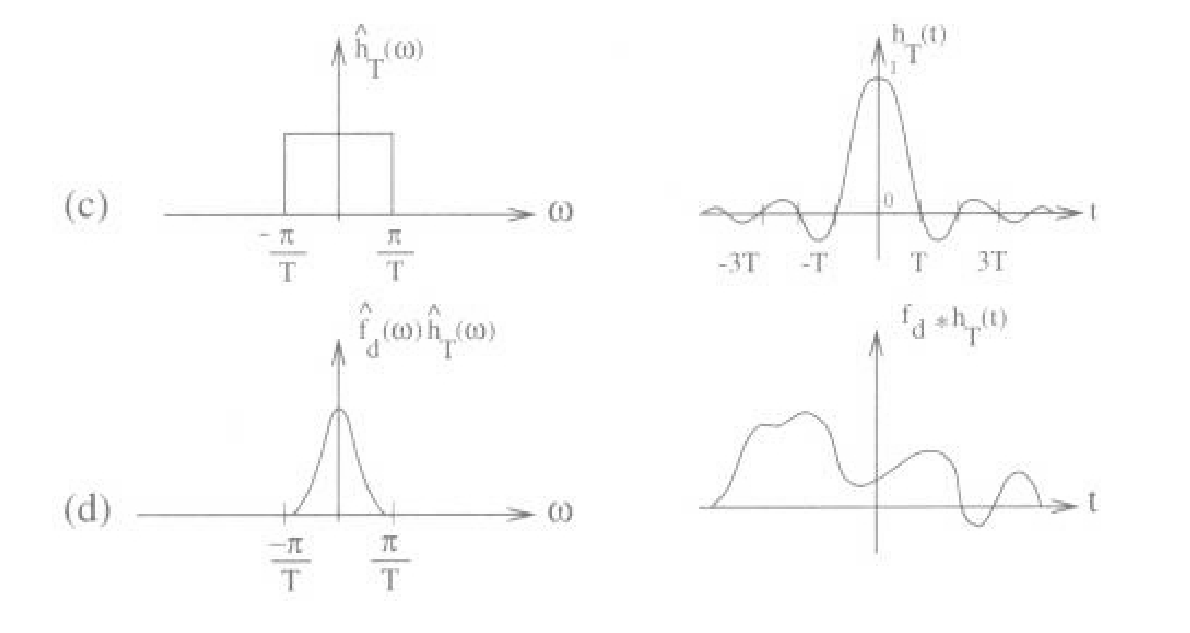
\includegraphics[width=10cm]{imatges/reconstruction.eps}
\caption{
%\cite{Mallat}.
[Mallat].
Reconstrucci\'o del senyal de la figura \ref{samplingFT.fig} a partir de les
seves mostres. (c) Funci\'o de reconstrucci\'o en el domini temporal
i freq\"uencial. (d) Resultat del producte de les transformades de $h_T$
i de $\hat{f}$ i senyal reconstruida. Observar com el senyal reconstruit
coincideix amb el senyal original.}
\label{mostreigOk.fig}
\end{center}
\end{figure}   

\begin{figure}[htbp]
\begin{center}
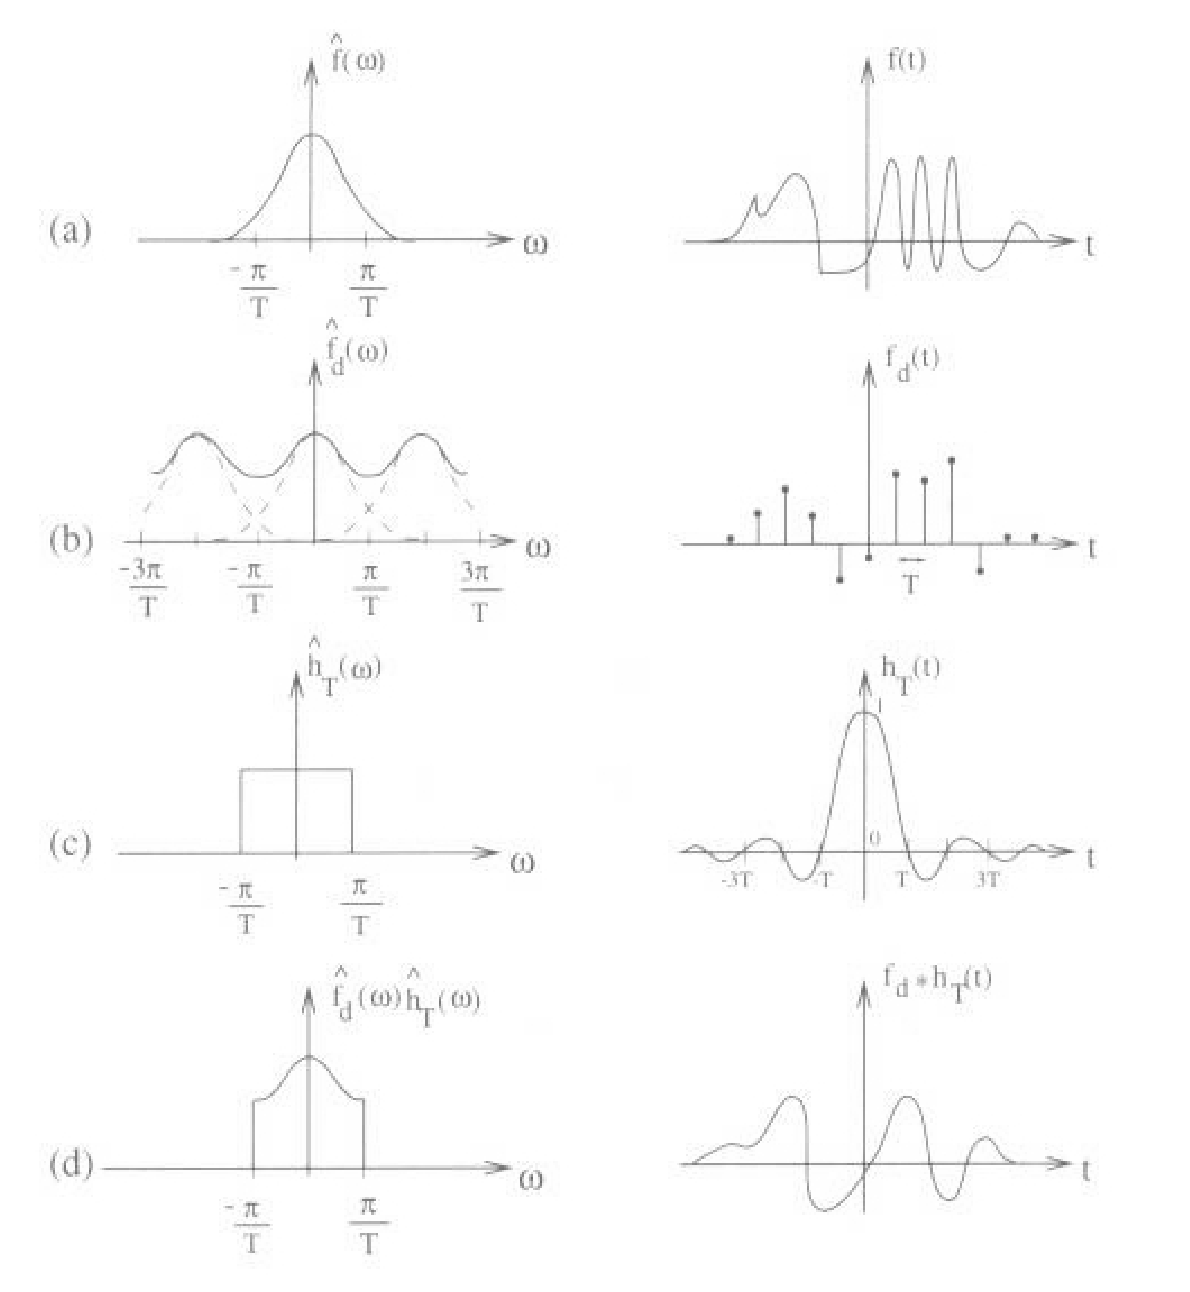
\includegraphics[width=10cm]{imatges/aliasing.eps}
\caption{
%\cite{Mallat}.
[Mallat].
(a) Senyal original i la seva transformada de Fourier.
(b) Senyal discret obtingut amb un per\'\i ode de mostreig que
no verifica les condicions del Teorema de Shannon. Observar el solapament
de funcions a nivell freq\"uencial (aliasing).
(c) Funci\'o de reconstrucci\'o en el domini temporal
i freq\"uencial. (d) Resultat del producte de les transformades de $h_T$
i de $\hat{f}$ i senyal reconstruida. Observar com el senyal reconstruit
\underline{no} coincideix amb el senyal original: les variacions
r\`apides han estat eliminades.}
\label{aliasing.fig}
\end{center}
\end{figure}  
 
\newpage
\section{Transformada Discreta de Fourier}
Ens plantejam en aquesta secci\'o el problema de calcular la transformada de
Fourier d'un senyal discret $x[n]$ format per $N$ mostres del senyal continu
$x(t)$.
Com ja s'ha raonat a la secci\'o \ref{mostreig}, la transformada de Fourier
d'una funci\'o discreta $x_d(t)=\sum_{n=-\infty}^{+\infty} x[n] \delta(t-nT)$,
v\'e donada per l'expressi\'o
\[
\hat{x}_d(\xi)=\sum_{n=-\infty}^{+\infty} x[n] e^{-i 2 \pi \xi n T}=
\sum_{n=-\infty}^{+\infty} \hat{x}(\xi-\frac{n}{T})
\]
\noindent
on $T$ \'es el per\'\i ode de mostreig, $x[n]=x(nT)$ i $\hat{x}(\xi)$ 
la transformada de 
Fourier del senyal continu original. 
$\hat{x}_d(\xi)$ \'es una funci\'o peri\`odica de per\'\i ode 
$\frac{1}{T}$.

Si consideram que el suport del senyal continu original est\'a compr\'es 
entre $0$ i $a$, i que les $N$ mostres s'han agafat equiespaiades, tendrem
que el per\'\i ode de mostreig \'es $T=\frac{a}{N}$ i l'equaci\'o anterior
es pot escriure de la seg\"uent manera:
\[
\hat{x}_d(\xi)=\sum_{n=0}^{N-1} x[n] e^{-i 2 \pi \xi n \frac{a}{N}}
\]
\noindent
a m\'es el per\'\i ode de $\hat{x}_d(\xi)$ ser\`a $\frac{N}{a}$, \'es a dir,
la funci\'o queda totalment determinada pels valors que pren entre $0$ i 
$\frac{N}{a}$. Si en aquest interval prenim $N$ mostres equiespaiades
obtenim una nova funci\'o discreta:
\begin{equation}
\label{DFT}
\hat{x}[k]=\hat{x}_d(\frac{k}{a})=\sum_{n=0}^{N-1} x[n] e^{-i 2 \pi n \frac{k}{N}}
\qquad k=0,\cdots, N-1 
\end{equation}
\noindent
$\hat{x}[k]$ \'es per tant una versi\'o discreta de $\hat{x}_d(\xi)$, on les mostres
s'han agafat per a valors de $\xi\in\{0, \frac{1}{a}, \cdots, \frac{N-1}{a}\}$.
Aquesta funci\'o rep el nom de {\bf Transformada Discreta de Fourier}  
(o {\bf DFT}) de $x[n]$.

\vskip 0.5 cm
Ens plantejam ara el problema invers a l'anterior: volem calcular la transformada
inversa de Fourier a partir de $N$ mostres d'una funci\'o $\widehat{x'}(\xi)$.
El problema \'es molt similar a l'anterior i podem fer el mateix raonament.

Consideram la funci\'o discreta en freq\"u\`encia 
$\widehat{x'}_d(\xi)=\sum_{k=-\infty}^{+\infty} \widehat{x'}[k] \delta(\xi-k T_\xi)$,
on $T_{\xi}$ \'es el per\'\i ode de mostreig en freq\"u\`encia.
Volem calcular la seva transformada de Fourier inversa. Fent un c\`alcul
molt similar al de la secci\'o \ref{mostreig} obtenim les seg\"uents expressions:
\[
x'_d(t)=\sum_{k=-\infty}^{+\infty} \widehat{x'}[k] e^{i 2 \pi t k T_\xi}=
\sum_{k=-\infty}^{+\infty} x'(t-\frac{k}{T_\xi})
\]
\noindent
on $\widehat{x'}[k]=\widehat{x'}(k T_\xi)$ i $x'(t)$ \'es la transformada inversa de 
Fourier del senyal continu $\hat{x'}(\xi)$.
$x'_d(t)$ \'es una funci\'o peri\`odica en temps, amb per\'iode $\frac{1}{T_\xi}$.

Si consideram que el suport de la funci\'o $\widehat{x'}(\xi)$ est\'a compr\`es entre
les freq\"u\`encies $-\frac{\xi_M}{2}$ i $\frac{\xi_M}{2}$ i que les $N$ mostres
s'han pres equiespaiades, llavors $T_\xi=\frac{\xi_M}{N}$ i les expressions anteriors
s'escriuen com
\begin{equation}
\label{idftcont}
x'_d(t)=\sum_{k=-\frac{N}{2}}^{+\frac{N}{2}} \widehat{x'}[k] e^{i 2 \pi t k \frac{\xi_M}{N}}
\end{equation}
Aquesta \'es una funci\'o peri\`odica qu\`e podem mostrejar amb $N$ valors equiespaiats
en el seu per\'\i ode principal (entre $0$ i $\frac{\xi_M}{N}$). Obtenim la funci\'o
discreta seg\"uent:
\[
x'[n]=x'_d(\frac{n}{\xi_M})=
\sum_{k=-\frac{N}{2}}^{+\frac{N}{2}} \widehat{x'}[k] e^{i 2 \pi k \frac{n}{N}}
\qquad n=0,\cdots, N-1
\]

Podem reescriure aquesta equaci\'o si fem les seg\"uents consideracions: 
suposam que les mostres de $\widehat{x'}(\xi)$ s'han guardat en un vector amb
indexos positius
tal que les mostres corresponents a freq\"u\`encies negatives ocupen les posicions
$\frac{N}{2}$ (el valor $\widehat{x'}_d(-\frac{N}{2}T_\xi)$), 
$\frac{N}{2}+1$ (el valor $\widehat{x'}_d((-\frac{N}{2}+1)T_\xi)$), i aix\'\i $ $ 
successivament fins a la posici\'o $N-1$ per al valor $\widehat{x'}_d(-1)$.
A m\'es, tenim que $e^{i 2 \pi k \frac{n}{N}}$ \'es una funci\'o peri\`odica de
per\'\i ode $N$. De manera que la f\`ormula anterior es pot escriure com:
\[
x'[n]=\sum_{k=0}^{N-1} \widehat{x'}[k] e^{i 2 \pi k \frac{n}{N}}
\]
Anomenam {\bf Transformada Inversa Discreta de Fourier} (o {\bf IDFT}) de 
$\widehat{x'}[k]$
a l'expressi\'o anterior multiplicada per un factor constant $\frac{1}{N}$:
\begin{equation}
\label{IDFT}
x'[n]=\frac{1}{N} \sum_{k=0}^{N-1} \widehat{x'}[k] e^{i 2 \pi k \frac{n}{N}}
\qquad n=0,\cdots,N-1
\end{equation}

\vskip 0.5 cm
Per acabar aquesta secci\'o estudiar la relacio entre les equacions (\ref{DFT})
i (\ref{IDFT}). \'Es a dir, podem afirmar que IDFT\{DFT\{$x[n]$\}\}=$x[n]$?.
\newline
I que DFT\{IDFT\{$\hat{x}[k]$\}\}=$\hat{x}[k]$?

Respecte a la primera pregunta, si consideram que el mostreig de $x[n]$ s'ha
fet respectant les condicions del teorema de Shannon, llavors la DFT, com a 
versi\'o mostrejada de la transformada de Fourier del senyal discret,
no presenta aliasing. Per tant, la DFT \'es igual a una versi\'o discreta de la
transformada de Fourier del senyal original i el resultat d'aplicar-li la IDFT
ser\`a un senyal id\`entic a l'original.

Per\`o qu\`e passa si el mostreig de $x[n]$ no cumpleix les condicions de Shannon?
En aquest cas, el senyal continu obtingut en aplicar l'equaci\'o (\ref{idftcont})
als valors de la DFT \'es diferent del senyal continu $x(t)$ original. No obstant 
aix\'o, la seg\"uent proposici\'o ens diu que en els punts de discretitzaci\'o
ambd\'os senyals prenen els mateixos valors.

\vskip 0.2 cm
\noindent
{\bf Proposici\'o}. Per a qualsevol senyal discret $x[n]$ es cumpleix 
$x[n]$=IDFT\{DFT\{$x[n]$\}\}.

\noindent
{\it Dem}. Sigui $\hat{x}[k]$=DFT{$x[n]$} i $x'[n]$=IDFT{$\hat{x}[k]$}. Hem 
de demostrar que $x'[n]=x[n]$, $\forall n \in \{0,\cdots,N-1\}$.

\noindent
Tenim que
\[
\begin{array}{rcl}
x'[n] & = & \frac{1}{N} \sum_{k=0}^{N-1} \hat{x}[k] e^{i 2 \pi k \frac{n}{N}}=
\frac{1}{N} \sum_{k=0}^{N-1} \left( 
\sum_{m=0}^{N-1} x[m] e^{-i 2 \pi m \frac{k}{N}} \right) e^{i 2 \pi k \frac{n}{N}} =\\ \\
& = & \frac{1}{N} \sum_{m=0}^{N-1} x[m] \left( \sum_{k=0}^{N-1} 
e^{i 2 \pi k \frac{n-m}{N}} \right)
\end{array}
\]
\noindent
el sumatori entre par\`entesi val $N$ quan $m=n$ i $0$ per a la resta de valors de $m$,
per tant $x'[n]=\frac{1}{N} x[n] N=x[n]$.
\begin{flushright}
$\square$
\end{flushright}

\vskip 0.2 cm
Seguint un raonament similar podem demostrar que tamb\'e es cumpleix la igualtat 
DFT\{IDFT\{$\hat{x}[k]$\}\}=$\hat{x}[k]$. 


\vskip 0.5 cm
{\bf Observacions}.
\begin{itemize}
\item Les funcions discretes obtingudes del c\`alcul de la DFT o la IDFT s\'on sempre 
funcions peri\`odiques, de per\'\i ode $N$.
\item Si definim $D_N$ com el conjunt de les funcions discretes peri\`odiques, de 
per\'\i ode $N$, formades per $N$ mostres equiespaiades, llavors la fam\'\i lia
de funcions $e_k[n]=e^{i 2 \pi \frac{k}{N}n}$ s\'on base de $D_N$. Podem intrepretar 
la IDFT com l'expressi\'o de $x[n]$ en aquesta base, de manera que les components de
$x[n]$ en la base s\'on la DFT.
\end{itemize}


\subsection{Transformada r\`apida de Fourier (FFT)}
El c\`alcul de la DFT per a senyals formats per moltes mostres \'es lent, de l'ordre 
de $N^2$ operacions (entre sumes i multiplicacions) per a un senyal de $N$ mostres.
Per exemple, si $N=262144$ (nombre de mostres que correspon a una imatge de tamany
mitj\`a, de $512 \times 512$ p\'\i xels), llavors el c\`alcul de la DFT necessita
m\'es de $6.87 \times 10^{10}$ operacions. Fa uns anys, quan els ordinadors m\'es r\`apids
tenien processadors de 1 MHz, el temps de c\`alcul hauria estat del voltant de 
$6.87 \times 10^10 \times 10^{-6} \approx 19$ hores!! 

Actualment els ordinadors s\'on m\'es r\`apids i poden tardar alguns minuts en calcular
la DFT. No obstant, el processament digital d'imatges no s'hagu\'es desenvolupat fins 
al punt que l'ha fet si en 1965 J.W.Cooley i J.W.Tuckey no hagu\`essin inventat un
algoritme r\`apid per al c\`alcul de la DFT, l'anomenat FFT (Fast Fourier Transform).
Podem dir sense cap mena de dubte que la revoluci\'o digital de les darreres d\`ecades deu molt
a aquest algoritme.

La FFT permet calcular la transformada discreta de Fourier d'un senyal de $N$ mostres
emprant $N log_2 N$ operacions. Per a l'exemple anterior amb $N=262144$ aix\'o implica unes
$4718592$ operacions que es poden realitzar en $4.7$ segons amb un ordinador amb processador
de 1 MHz (comparat amb les 19 hores de l'algoritme original!!).

Una versi\'o senzilla de la FFT, qu\`e serveix quan $N$ \'es una pot\`encia de $2$ 
($N=2^m$), \'es la seg\"uent:

Per a les freq\"u\`encies parells s'agrupen els termes $n$ i $n+\frac{N}{2}$:
\begin{equation}
\label{FFTparell}
\hat{x}[2k]=\sum_{n=0}^{\frac{N}{2}-1} (x[n]+x[n+\frac{N}{2}]) e^{-i 2 \pi \frac{k n}{N/2}}
\end{equation}

\noindent
per a les freq\"u\`encies imparells tamb\'e agrupam els termes $n$ i $n+\frac{N}{2}$:
\begin{equation}
\label{FFTimparell}
\hat{x}[2k+1]=\sum_{n=0}^{\frac{N}{2}-1} e^{-i 2 \pi \frac{n}{N}} 
(x[n]-x[n+\frac{N}{2}]) e^{-i 2 \pi \frac{k n}{N/2}}
\end{equation}

Ara b\'e, (\ref{FFTparell}) \'es la DFT del senyal peri\`odic $x[n]+x[n+\frac{N}{2}]$
i (\ref{FFTimparell}) \'es la DFT de $e^{-i 2 \pi \frac{n}{N}} (x[n]-x[n+\frac{N}{2}])$.
De manera que la DFT de $x[n]$ se calcula com 2 DFT de senyals amb la meitat de mostres.
Repetint el proc\'es de divisi\'o del senyal en senyals de tamany cada vegada m\'es
petit arribam a un algoritme de c\`alcul amb $N log_2 N$ operacions.


\subsection{Transformada Discreta de Fourier en 2D}
Una part molt important del tractament del senyal est\`a orientada al tractament 
d'imatges, \'es necessari per tant adaptar l'an\`alisi del senyal discret al cas
bidimensional.

En l'apartat \ref{TFbidimensional} hem vist les expressions de les transformades de Fourier
directa i inversa en el cas bidimensional. Anam ara a estudiar la discretitzaci\'o 
d'aquestes expressions.

Sigui $f_d(x,y)$ la versi\'o discreta de $f(x,y)$:
\[
f_d(x,y)=\begin{cases} f(x,y) & \mathrm{si} \, x=nT_1 \, \mathrm{i} \, y=mT_2
\quad n,m \in \Z \\
0 & \mathrm{altrament}
\end{cases}
\]
\noindent
llavors podem escriure $f_d$ en funci\'o de les deltes de Dirac com
\[
f_d(x,y)=\sum_{n,m=-\infty}^{\infty} f(nT_1, mT_2) \delta(x-nT_1) \delta(y-mT_2)
\]
\noindent
i podem aplicar el mateix an\`alisi fet en una dimensi\'o per obtenir:
\[
\hat{f}_d(\xi_1, \xi_2)=\frac{1}{T_1 T_2} \sum_{k_1, k_2=-\infty}^{\infty} 
\hat{f}(\xi_1-\frac{k_1}{T_1}, \xi_2-\frac{k_2}{T_2})
\]

\'Es a dir, hi ha una perioditzaci\'o de l'espectre de $\hat{f}$ en les direccions
$\xi_1$ i $\xi_2$.

\begin{figure}[htbp]
\begin{center}
\begin{tabular}{cc}
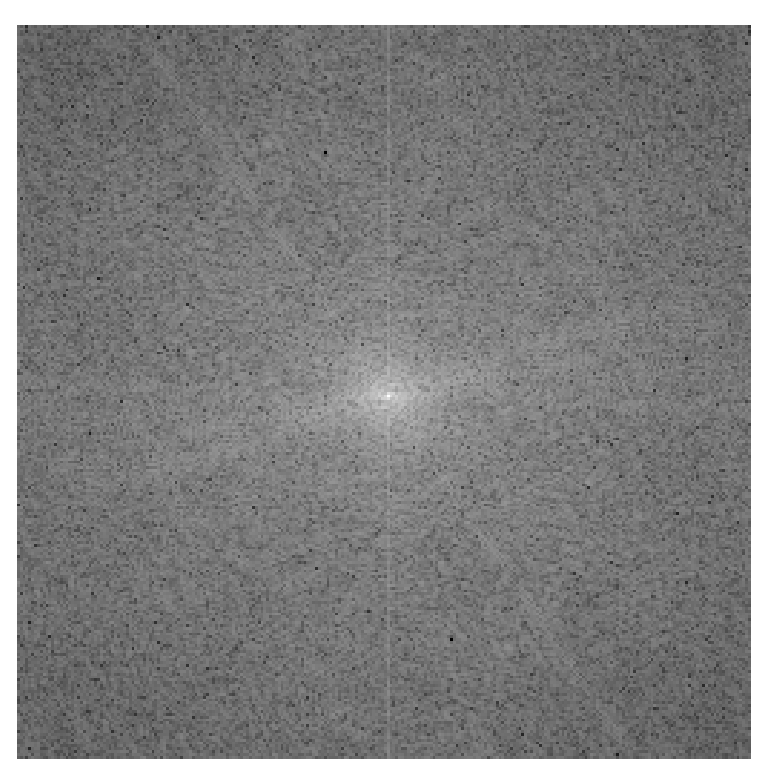
\includegraphics[width=1.75cm]{imatges/espectre2D.eps} &
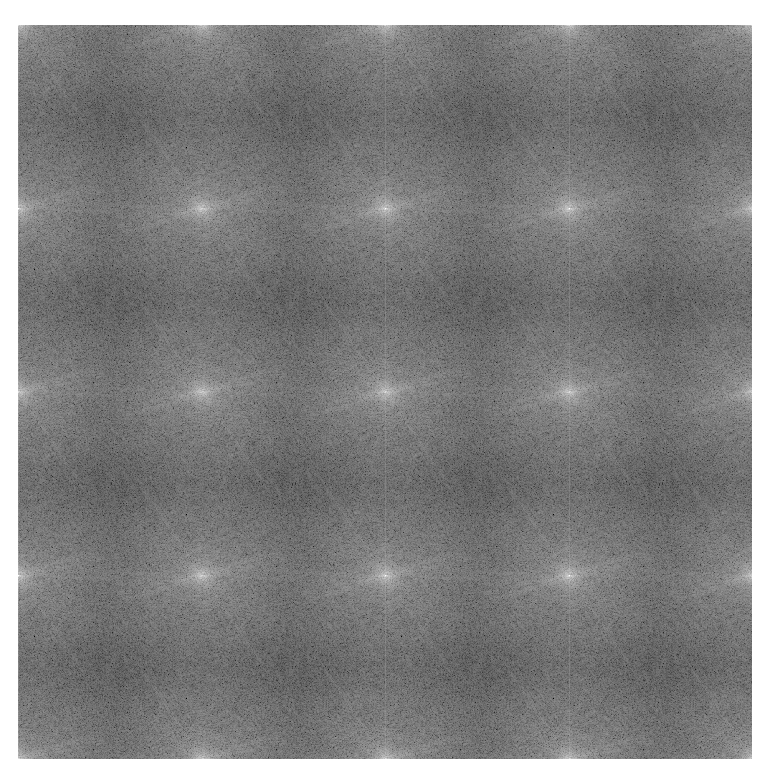
\includegraphics[width=7cm]{imatges/espectre2Dm.eps}
\end{tabular}
\caption{Esquerra, m\`odul de la transformada de Fourier d'un senyal continu 
bidimensional.
Dreta, m\`odul de la transformada de Fourier d'un senyal discret bidimensional.}
\end{center}
\end{figure}

En el cas bidimensional, per evitar l'aliasing, el suport de $\hat{f}$ ha d'estar
contingut en $[-\frac{1}{2T_1}, \frac{1}{2T_1}] \times [-\frac{1}{2T_2}, \frac{1}{2T_2}]$
({\bf condici\'o de Shannon per a senyals bidimensionals}).

\subsubsection{DFT bidimensional}
Sigui $f[n,m]$ un senyal bidimensional format per $N$ mostres en la direcci\'o $x$ i 
$M$ mostres en la direcci\'o $y$. La transformada discreta de Fourier de $f$ \'es
\begin{equation}
\label{DFT2D}
\hat{f}[k_1, k_2]=\sum_{n=0}^{N-1} \sum_{m=0}^{M-1} f[n,m] 
e^{-i 2 \pi (k_1 \frac{n}{N} + k_2 \frac{m}{M})}
\end{equation}

La transformada inversa se calcula com
\begin{equation}
f[n,m]=\frac{1}{N}\frac{1}{M} \sum_{k_1=0}^{N-1} \sum_{k_2=0}^{M-1} \hat{f}[k_1,k_2] 
e^{i 2 \pi (k_1 \frac{n}{N} + k_2 \frac{m}{M})}
\end{equation}

\vskip 0.3 cm
\noindent
{\bf Propietat}. \'Es possible calcular la DFT (resp. IDFT) bidimensional  
a partir de la DFT (resp. IDFT) en una dimensi\'o.

\noindent
{\it Dem}. Podem descomposar l'equaci\'o (\ref{DFT2D}) de la seg\"uent
manera:
\[
\hat{f}[k_1,k_2]=\sum_{n=0}^{N-1} \left( \sum_{m=0}^{M-1} f[n,m]
e^{-i 2 \pi k_2 \frac{m}{M}} \right) e^{-i 2 \pi k_1 \frac{n}{N}}
\]
L'expressi\'o entre par\`entesi \'es la DFT unidimensional de $f$ quan $n$
est\'a fixat. Si anomenam a aquesta expressi\'o $f'[n,k_2]$, llavors
\[
\hat{f}[k_1,k_2]= \sum_{n=0}^{N-1} f'[n,k_2] e^{-i 2 \pi k_1 \frac{n}{N}}
\]
\noindent
qu\`e \'es la DFT unidimensional de $f'[n,k_2]$, per a cada valor de $n$.
\begin{flushright}
$\square$
\end{flushright}

\vskip 0.3 cm
La propietat anterior implica que el c\`alcul de la DFT en dues dimensions es
pot fer aplicant els mateixos algoritmes explicats en els apartats anteriors.
En particular, es pot emprar l'algotitme de la FFT.






 

\end{document} 